%% ================================================================
%% Artigo Cienciométrico -- Ligas de Alta Entropia para Aplicações Hipersônicas
%% Arquitetura Modular / Clean Code
%% Compilar: pdflatex main.tex
%% ================================================================

%% ================================================================
%% Artigo Cienciométrico -- Ligas de Alta Entropia para Aplicações Hipersônicas
%% Configurações e Preâmbulo -- Padrão Moderno Overleaf / Academic Template
%% ================================================================
\documentclass[11pt,a4paper]{article}

%% ---------------- Codificação e Fontes
\usepackage[utf8]{inputenc}
\usepackage[T1]{fontenc}
\usepackage{textcomp}
\usepackage{lmodern}

%% ---------------- Paleta de Cores Acadêmica Moderna (Overleaf Style)
\usepackage{color}
\definecolor{primary}{rgb}{0.07, 0.21, 0.42}       % Deep Navy / Azul Marinho Nobre
\definecolor{secondary}{rgb}{0.18, 0.40, 0.62}     % Slate Blue / Azul Médio
\definecolor{accent}{rgb}{0.65, 0.15, 0.15}        % Dark Crimson / Destaque sutil
\definecolor{linegray}{rgb}{0.80, 0.84, 0.90}      % Linha divisória suave
\definecolor{boxbg}{rgb}{0.96, 0.97, 0.99}        % Fundo suave para caixas de resumo
\definecolor{tablehead}{rgb}{0.90, 0.93, 0.97}     % Fundo para cabeçalho de tabelas

%% ---------------- Geometria e Espaçamento de Página
\usepackage[top=2.5cm,bottom=2.5cm,left=2.5cm,right=2.5cm,headheight=14.5pt]{geometry}
\renewcommand{\baselinestretch}{1.18}               % Entrelinha arejada e agradável à leitura
\setlength{\parindent}{1.0cm}                       % Recuo padrão elegante
\setlength{\parskip}{3pt plus 1pt minus 1pt}        % Leve espaçamento entre parágrafos
\usepackage{indentfirst}

%% ---------------- Cabeçalhos e Rodapés Dinâmicos (fancyhdr)
\usepackage{fancyhdr}
\pagestyle{fancy}
\fancyhf{}
\fancyhead[L]{\small\textsf{\color{secondary} Estudo Cienciométrico --- Ligas de Alta Entropia para Voo Hipersônico}}
\fancyhead[R]{\small\textsf{\bfseries\color{primary} \thepage}}
\renewcommand{\headrulewidth}{0.5pt}
\renewcommand{\headrule}{{\color{linegray}\hrule height \headrulewidth \vspace{2pt}}}
\renewcommand{\footrulewidth}{0pt}

%% Estilo limpo para primeira página
\fancypagestyle{plain}{%
  \fancyhf{}%
  \fancyfoot[C]{\small\textsf{\color{secondary} \thepage}}%
  \renewcommand{\headrulewidth}{0pt}%
}

%% ---------------- Nomes em Português
\renewcommand{\abstractname}{Resumo}
\renewcommand{\figurename}{Figura}
\renewcommand{\tablename}{Tabela}
\renewcommand{\refname}{Referências Bibliográficas}

%% ---------------- Matemática, Gráficos e Tabelas
\usepackage{amsmath,amssymb}
\usepackage{graphicx}
\usepackage{tabularx}
\usepackage{array}
\usepackage{multicol}

%% ---------------- Macros de compatibilidade e elegância para tabelas
\providecommand{\toprule}{\hline\hline}
\providecommand{\midrule}{\hline}
\providecommand{\bottomrule}{\hline\hline}

%% ---------------- Legenda de Figuras e Tabelas
\newcommand{\legend}[1]{\par\vspace{4pt}{\footnotesize\color{secondary}\centering\textsf{#1}\par}\vspace{6pt}}

%% ---------------- Citação longa em bloco
\newenvironment{citacao}
  {\par\vspace{0.6em}\begin{list}{}{\setlength{\leftmargin}{3.5cm}\setlength{\rightmargin}{0.5cm}\setlength{\parsep}{0pt}\setlength{\topsep}{0pt}}
   \item[]\small\color{primary}\renewcommand{\baselinestretch}{1.05}\selectfont}
  {\end{list}\vspace{0.6em}}

%% ---------------- Tipografia de Títulos (Estilo Editorial Overleaf)
\makeatletter
\renewcommand{\section}{\@startsection{section}{1}{\z@}%
  {-3.5ex \@plus -1ex \@minus -.2ex}%
  {1.8ex \@plus.2ex}%
  {\normalfont\Large\bfseries\color{primary}}}

\renewcommand{\subsection}{\@startsection{subsection}{2}{\z@}%
  {-2.8ex\@plus -1ex \@minus -.2ex}%
  {1.2ex \@plus .2ex}%
  {\normalfont\large\bfseries\color{secondary}}}

\renewcommand{\subsubsection}{\@startsection{subsubsection}{3}{\z@}%
  {-2.2ex\@plus -1ex \@minus -.2ex}%
  {0.8ex \@plus .2ex}%
  {\normalfont\normalsize\bfseries\color{primary}}}
\makeatother

%% ---------------- Links e URLs formatadas
\setlength{\leftmargini}{1.0cm}
\usepackage{url}
\urlstyle{sf}
\providecommand{\href}[2]{{\color{secondary}\underline{#2}}}

%% ---------------- Título e Autoria Estilizados
\title{\vspace{-1.5cm}%
  {\Huge\bfseries\color{primary} Estudo Cienciométrico Avançado sobre Ligas de Alta Entropia para Aplicações Hipersónicas}\\[0.35cm]
  {\Large\textsl{\color{secondary} Redes de Autoria, Artigos Seminais e Evolução do Conhecimento}}%
}
\author{%
  \textbf{Valber Marcelino Filho}\thanks{Instituto Militar de Engenharia / Pesquisador Principal} \quad\and\quad
  \textbf{Rodrigo Andrade Paes}\thanks{Orientador e Supervisor de Pesquisa}%
}
\date{\vspace{0.2cm}\small\textsf{\color{secondary} Outubro de 2026}}

%% ---------------- Formatação refinada de tabelas
\renewcommand{\arraystretch}{1.28}
\setlength{\tabcolsep}{6pt}


\begin{document}

\maketitle
\thispagestyle{plain}

%% ---------------- Resumo e Palavras-chave
\renewcommand{\abstractname}{\large\bfseries\color{primary} Resumo}
\begin{abstract}
\noindent As demandas severas de componentes de reentrada atmosférica e veículos hipersónicos exigem novos materiais capazes de manter integridade estrutural sob elevadas solicitações aerotérmicas, oxidativas e mecânicas. As Ligas de Alta Entropia (HEAs) e, em particular, as Ligas de Alta Entropia Refratárias (RHEAs) surgem como uma das fronteiras mais promissoras da engenharia de materiais de ultra-alta temperatura (UHT). Este trabalho apresenta um estudo cienciométrico e de revisão crítica estruturado sobre um modelo metodológico replicável. A partir de uma estratégia de busca combinatória automatizada via script Python cruzando 42 descritores de ligas e 22 descritores de severidade aerotérmica nos campos \texttt{TI OR AB OR AK} na \emph{Web of Science Core Collection} (período 2004--2026), consolidou-se um corpus macroscópico de 192 documentos de alta especialização. O estudo implementa rotinas de higienização de dados (\emph{thesaurus}) e mitigação do efeito de homonímia na desambiguação autoral (AND). Concomitantemente à caracterização quantitativa das frentes de publicação via Bibliometrix e VOSviewer, realiza-se a síntese qualitativa dos mecanismos de endurecimento, estabilidade de fases BCC/B2, limites de escoamento até 2000 \textdegree{}C e o compromisso crítico entre ductilidade a frio e resistência à oxidação/\emph{pesting} em regimes de Mach 5+.

\vspace{0.8em}
\noindent {\color{primary}\textbf{Palavras-chave:}} Ligas de Alta Entropia; Ligas de Alta Entropia Refratárias (RHEAs); Voo Hipersónico; Cienciometria; Arquitetura de Duplo Corpus (BACR); Desambiguação Autoral; Bibliometria.
\end{abstract}


\vspace{0.8cm}
\hrule
\vspace{0.8cm}

%% ---------------- Seções do Artigo
\section{Introdução}\label{sec:introducao}

O desenvolvimento de sistemas de propulsão e veículos para voo hipersónico (velocidades superiores a Mach 5) representa um dos maiores desafios contemporâneos da engenharia aeroespacial. Componentes expostos ao fluxo aerodinâmico extremo, tais como bordos de ataque, bordos de ataque de asas, dutos de admissão e sistemas de proteção térmica (TPS), enfrentam aquecimento atrito severo, resultando em temperaturas operacionais que superam facilmente 1500 \textdegree{}C, acompanhadas de gradientes térmicos acentuados e oxidação agressiva.

Superligas tradicionais à base de níquel ou cobalto atingem seus limites operacionais próximos de 1100 \textdegree{}C, enquanto cerâmicas ultra-refratárias (UHTCs), embora resistam a temperaturas elevadas, frequentemente sofrem com baixa tenacidade à fratura e suscetibilidade ao choque térmico. Nesse contexto, o paradigma das Ligas de Alta Entropia (HEAs), proposto em 2004, revolucionou o design de ligas metálicas ao explorar misturas equiatómicas ou quase-equiatómicas de cinco ou mais elementos principais.

Dentro desse domínio, as Ligas de Alta Entropia Refratárias (RHEAs) --- constituídas por elementos de alto ponto de fusão como Nb, Mo, Ta, W, Ti, Zr, V e Hf --- emergem como candidatas-chave para substituir superligas convencionais em ambientes de temperatura ultra-alta. Com a expansão acelerada dessa área de pesquisa, torna-se essencial quantificar e estruturar o conhecimento acumulado. Este trabalho realiza uma análise cienciométrica detalhada e revisão crítica a partir do corpus consolidado de 192 publicações altamente especializadas (período 2004--2026), mapeando a estrutura de autoria, artigos de alto impacto, citações locais e a base teórica estabelecida pelos pioneiros do campo.

\section{Metodologia}\label{sec:metodologia}

Para compreender a evolução das Ligas de Alta Entropia em regimes hipersônicos, este estudo desenvolveu um levantamento bibliométrico na base de dados \emph{Web of Science Core Collection} abrangendo o período de 2004 a 2026. O objetivo central consistiu em estruturar um protocolo transparente e determinístico, assegurando que pesquisadores independentes possam replicar integralmente cada etapa da triagem e recuperar os mesmos registros documentais.

\subsection{Estratégia de Busca e Combinação Booleana}\label{sec:estrategia_busca}

A formulação da expressão de busca assemelha-se ao ajuste focal de uma lente óptica, onde a amplitude excessiva capta ruídos irrelevantes e a restrição severa descarta dados essenciais. Enquanto buscas genéricas por propriedades mecânicas em alta temperatura retornam milhares de publicações desvinculadas da severidade aeroespacial, a conjunção direta e exclusiva das palavras ``HEAs'' e ``hipersônico'' recupera apenas 38 estudos, omitindo marcos fundamentais da termodinâmica de ligas refratárias.

Para superar essa limitação, desenhou-se uma estratégia combinatória automatizada em linguagem Python baseada no cruzamento de duas categorias temáticas completas. A primeira categoria congrega 42 variações terminológicas dedicadas a ligas de alta entropia, composicionalmente complexas e ligas refratárias concentradas (como HEAs, RHEAs, CCAs e MPEAs). A segunda categoria reúne 22 descritores técnicos associados a solicitações hipersônicas e condições extremas, incluindo propulsão \emph{scramjet}, configurações \emph{waverider}, ablação, choque térmico e ensaios em túneis de plasma. O algoritmo computacional gerou o produto cartesiano de todos os pares possíveis unidos pelo operador \texttt{AND}, articulando-os sequencialmente via \texttt{OR} sobre os campos de Título (\texttt{TI}), Resumo (\texttt{AB}) e Palavras-chave do Autor (\texttt{AK}). Essa parametrização filtrou com precisão cirúrgica um corpus consolidado de 192 artigos científicos altamente especializados, cujas listas completas de palavras estão documentadas no Apêndice~\ref{apendice:query_wos}.

\subsection{Higienização e Padronização dos Dados}\label{sec:elegibilidade_processamento}

Bancos de dados bibliográficos brutos apresentam inconsistências terminológicas e sobreposições autorais que exigem tratamento prévio rigoroso. Inicialmente, construiu-se um vocabulário controlado (\emph{thesaurus}) para unificar as múltiplas designações de materiais sob uma taxonomia estável, impedindo que variações acrônimas dispersassem núcleos de pesquisa semanticamente idênticos. 

Adicionalmente, enfrentou-se o desafio crítico da homonímia autoral decorrente da indexação abreviada de pesquisadores pelo padrão sobrenome-inicial. Nomes recorrentes na literatura asiática foram desambiguados manualmente através do cruzamento de identificadores digitais persistentes (ORCID e Scopus Author ID), análise do histórico de afiliações institucionais e correlação de redes de coautoria habitual. Definiram-se como critérios de elegibilidade a inclusão exclusiva de artigos originais e revisões por pares focados em comportamento mecânico, microestrutural ou oxidativo em temperaturas superiores a $1200~^\circ\mathrm{C}$ e condições de tocha ou plasma. Ligas diluídas convencionais ou estudos restritos a temperaturas moderadas foram descartados. A base depurada foi então processada de forma integrada no pacote \emph{Bibliometrix} (ambiente R) para extração de indicadores cronológicos e no software \emph{VOSviewer} para mapeamento e clusterização de redes colaborativas.

\section{Resultados e Discussão}\label{sec:resultados_discussao}



\subsection{Visão Geral do Corpus Científico e Evolução Bibliométrica}\label{visao-geral-do-corpus-cientifico-e-evolucao-bibliometrica}

A Tabela~\ref{tab:main_info} sintetiza os principais parâmetros estatísticos e descritivos do conjunto de dados atualizado, composto por 192 documentos recuperados e validados por pares na base de dados \emph{Web of Science} (WoS). O escopo temporal foi delimitado a partir de 2004, marco histórico da introdução formal do conceito de Ligas de Alta Entropia (HEAs). Observa-se uma taxa de crescimento anual composta (CAGR) robusta de 15.76\%, evidenciando a maturidade acelerada do campo, impulsionada pelo interesse estratégico em formulações refratárias e resistência a ambientes extremos.

\begin{table}[!htbp]
\centering
\caption{Informações Principais sobre o Conjunto de Dados Analisado (2004--2026)}\label{tab:main_info}
\small
\begin{tabularx}{\textwidth}{>{\raggedright\arraybackslash}X>{\raggedright\arraybackslash}X}
\toprule
\textbf{Descrição do Indicador Bibliométrico} & \textbf{Resultado Atualizado} \\
\midrule
Período Temporal Analisado & 2004 -- 2026 \\
Total de Documentos Recuperados & 192 \\
Taxa de Crescimento Anual Composta (CAGR) & 15.76\% \\
Idade Média dos Documentos & 2.47 anos \\
Periódicos e Fontes de Publicação Dominantes & \emph{J. Alloys Compd.}, \emph{Surf. Coat. Technol.}, \emph{Appl. Surf. Sci.} \\
Tipologia Documental Dominante & Artigos de Pesquisa Original e Revisões \\
\bottomrule
\end{tabularx}
\legend{Fonte: Elaborado pelos autores (2026), com base em dados da \emph{Web of Science}.}
\end{table}

A distribuição temporal da produção científica, ilustrada na Figura~\ref{fig:annual_production}, evidencia uma trajetória evolutiva claramente demarcada em quatro fases. O período inicial de latência e fundações conceituais (2004--2009) reuniu quatro publicações pioneiras que estabeleceram as bases teóricas da alta entropia configuracional antes da exploração ampla de misturas refratárias. A fase subsequente de formulação das RHEAs (2010--2014) delimitou os primeiros sistemas equiatômicos de elevado ponto de fusão e a exploração exploratória de ligas multicomponentes concentradas, registrando dois artigos representativos. Em seguida, a fase de prova de conceito e mapeamento de gargalos (2015--2019), com nove artigos, iniciou a avaliação termomecânica sistemática e evidenciou vulnerabilidades críticas, como oxidação catastrófica e \emph{pesting}. Por fim, a fase de expansão exponencial e direcionamento a regimes severos (2020--2026) congregou 176 artigos, atingindo 53 publicações em 2025 e 50 registros em 2026 até o término da coleta, impulsionada pela demanda urgente de materiais estruturais para voos hipersônicos (Mach 5+), escudos de reentrada e sistemas de propulsão scramjet.

\begin{figure}[!htbp]
\centering
\caption{Evolução da produção científica anual (2004--2026) no corpus consolidado de 192 documentos.}\label{fig:annual_production}
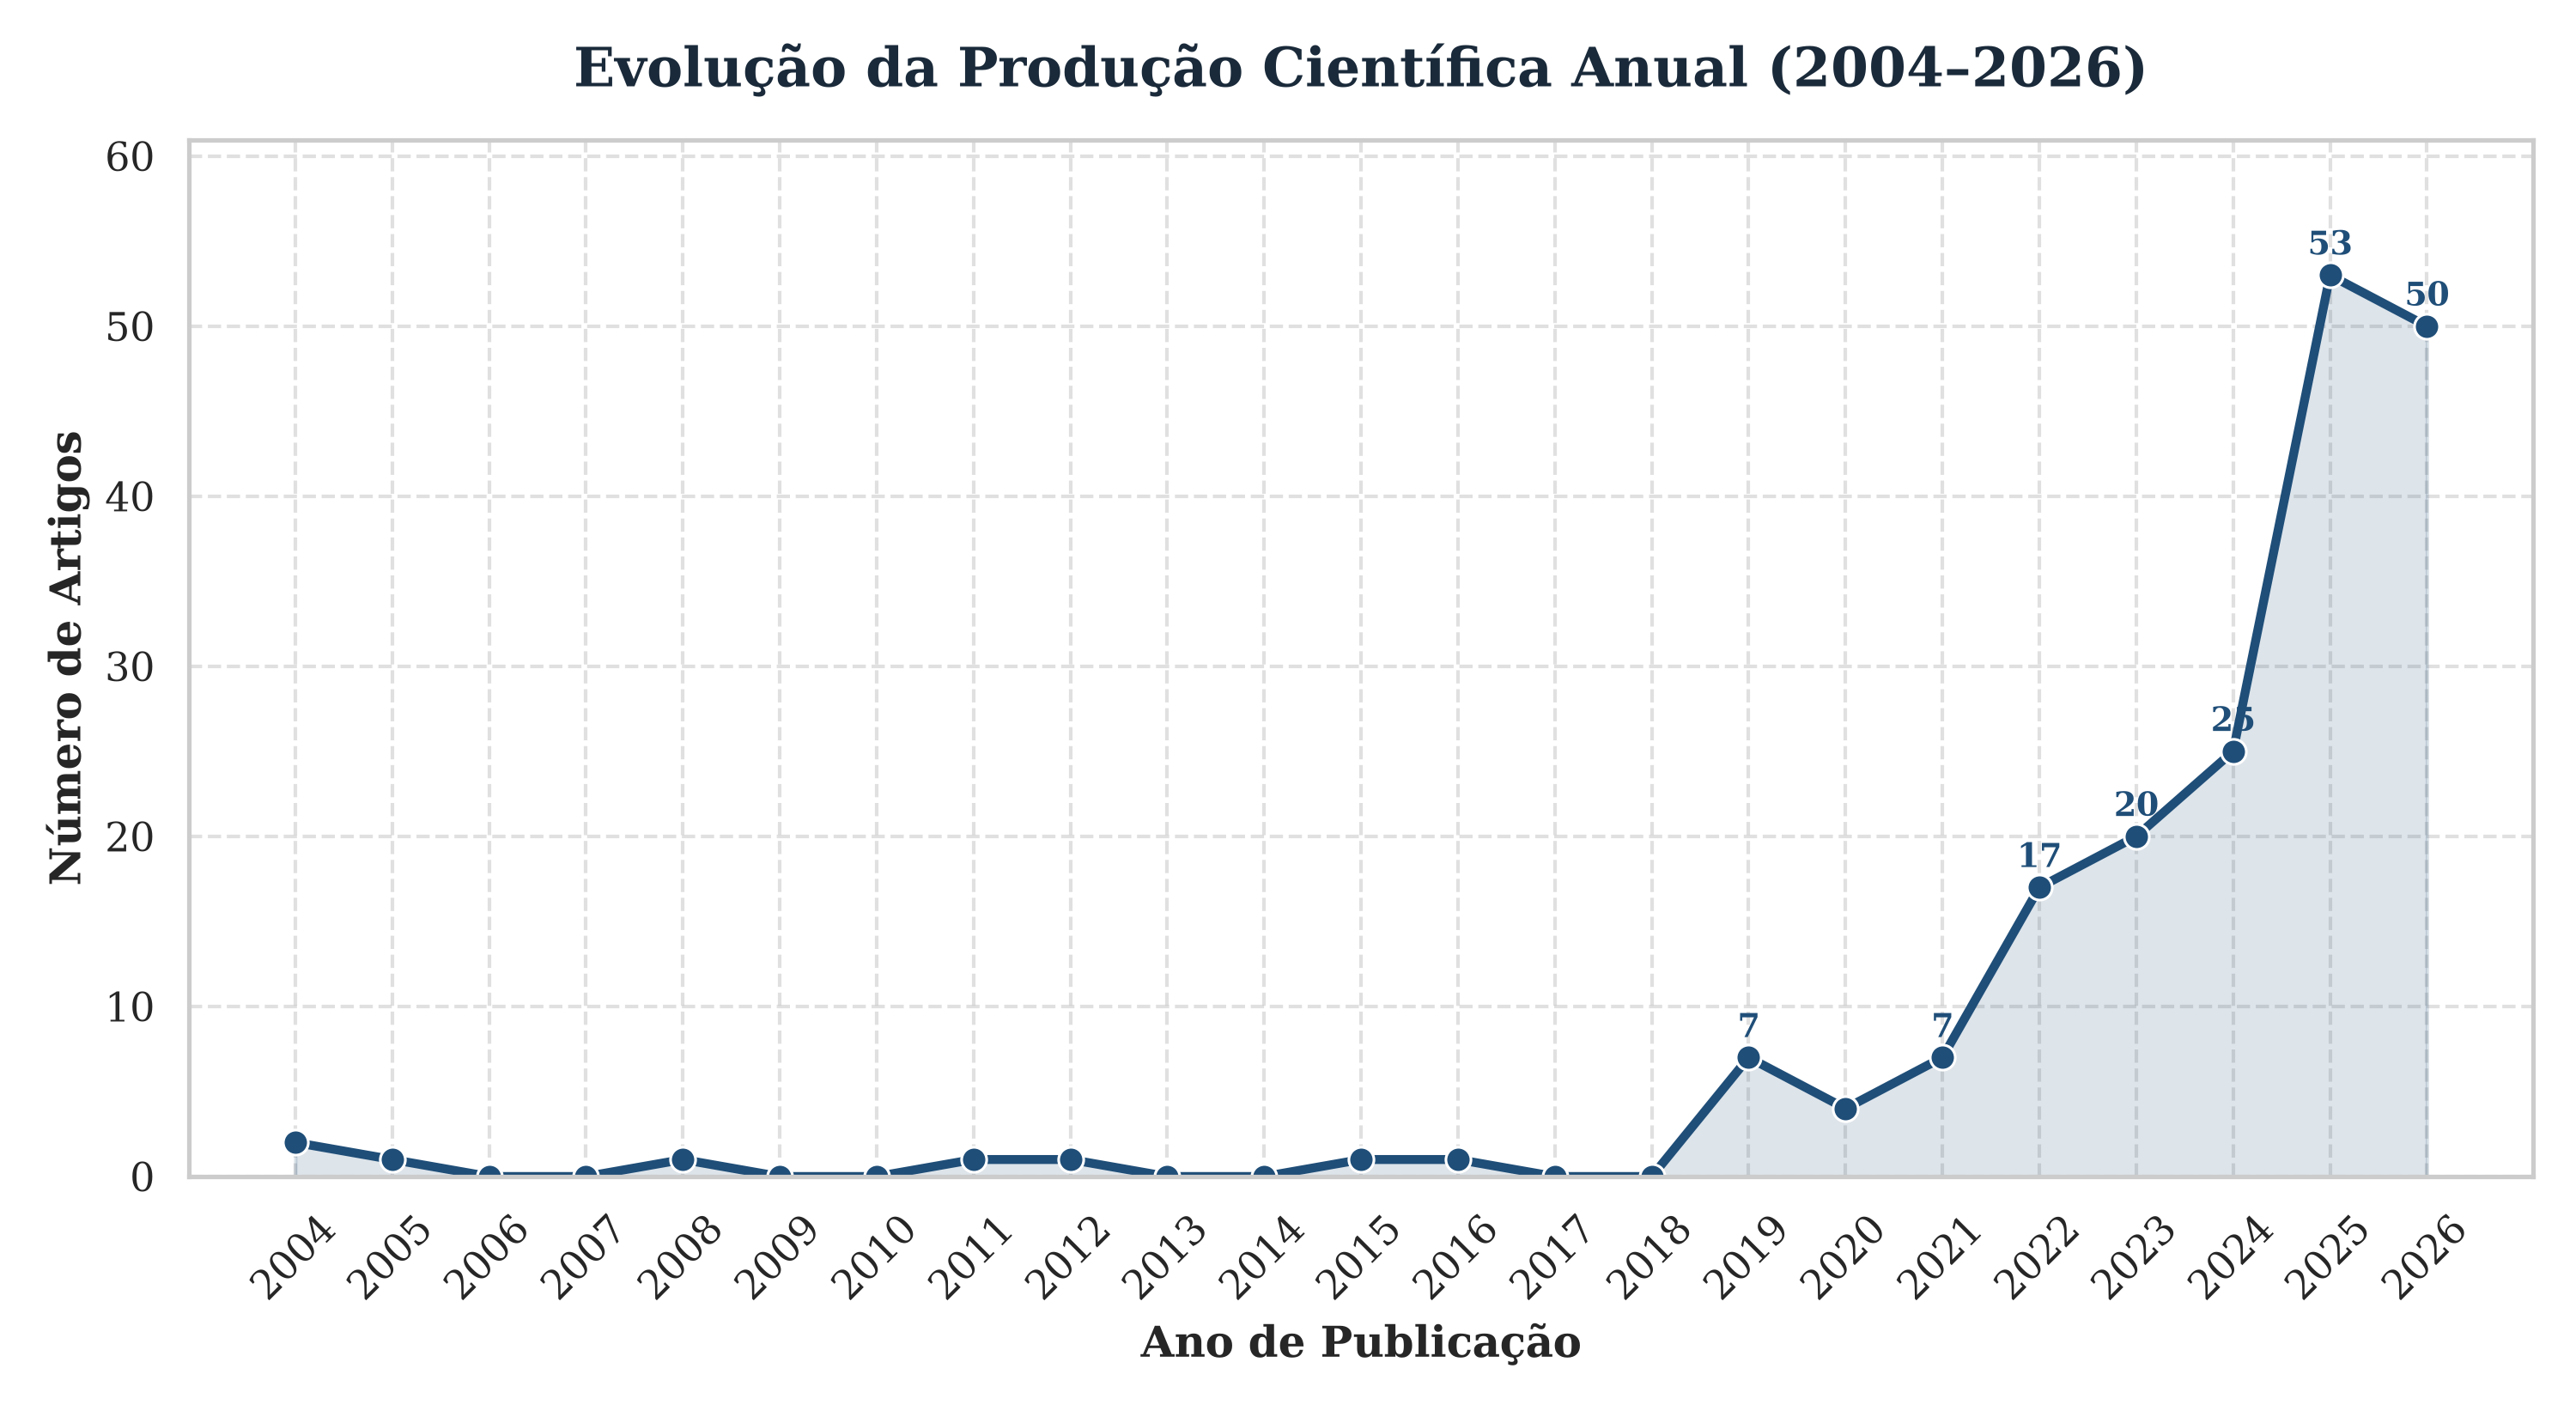
\includegraphics[width=0.85\textwidth]{figuras/annual_production.png}
\legend{Fonte: Elaborado pelos autores (2026), a partir de dados da \emph{Web of Science}.}
\end{figure}

\subsection{Perfil das Fontes de Publicação e Impacto Periódico}\label{perfil-das-fontes-de-publicacao-e-impacto-periodico}

O mapeamento das fontes de disseminação científica revela forte concentração em periódicos de alto impacto focados em física de superfícies, ciência dos materiais e revestimentos funcionais. A Figura~\ref{fig:relevant_sources} destaca as revistas científicas mais relevantes por volume de documentos publicados, lideradas pelo \emph{Journal of Alloys and Compounds} (12 artigos), seguido por \emph{Surface \& Coatings Technology} (7 artigos) e \emph{Applied Surface Science} (6 artigos), acompanhados por revistas de alto prestígio como \emph{Advanced Materials} (5 artigos) e \emph{Intermetallics} (5 artigos).

\begin{figure}[!htbp]
\centering
\caption{Periódicos mais relevantes em número absoluto de artigos publicados no corpus.}\label{fig:relevant_sources}
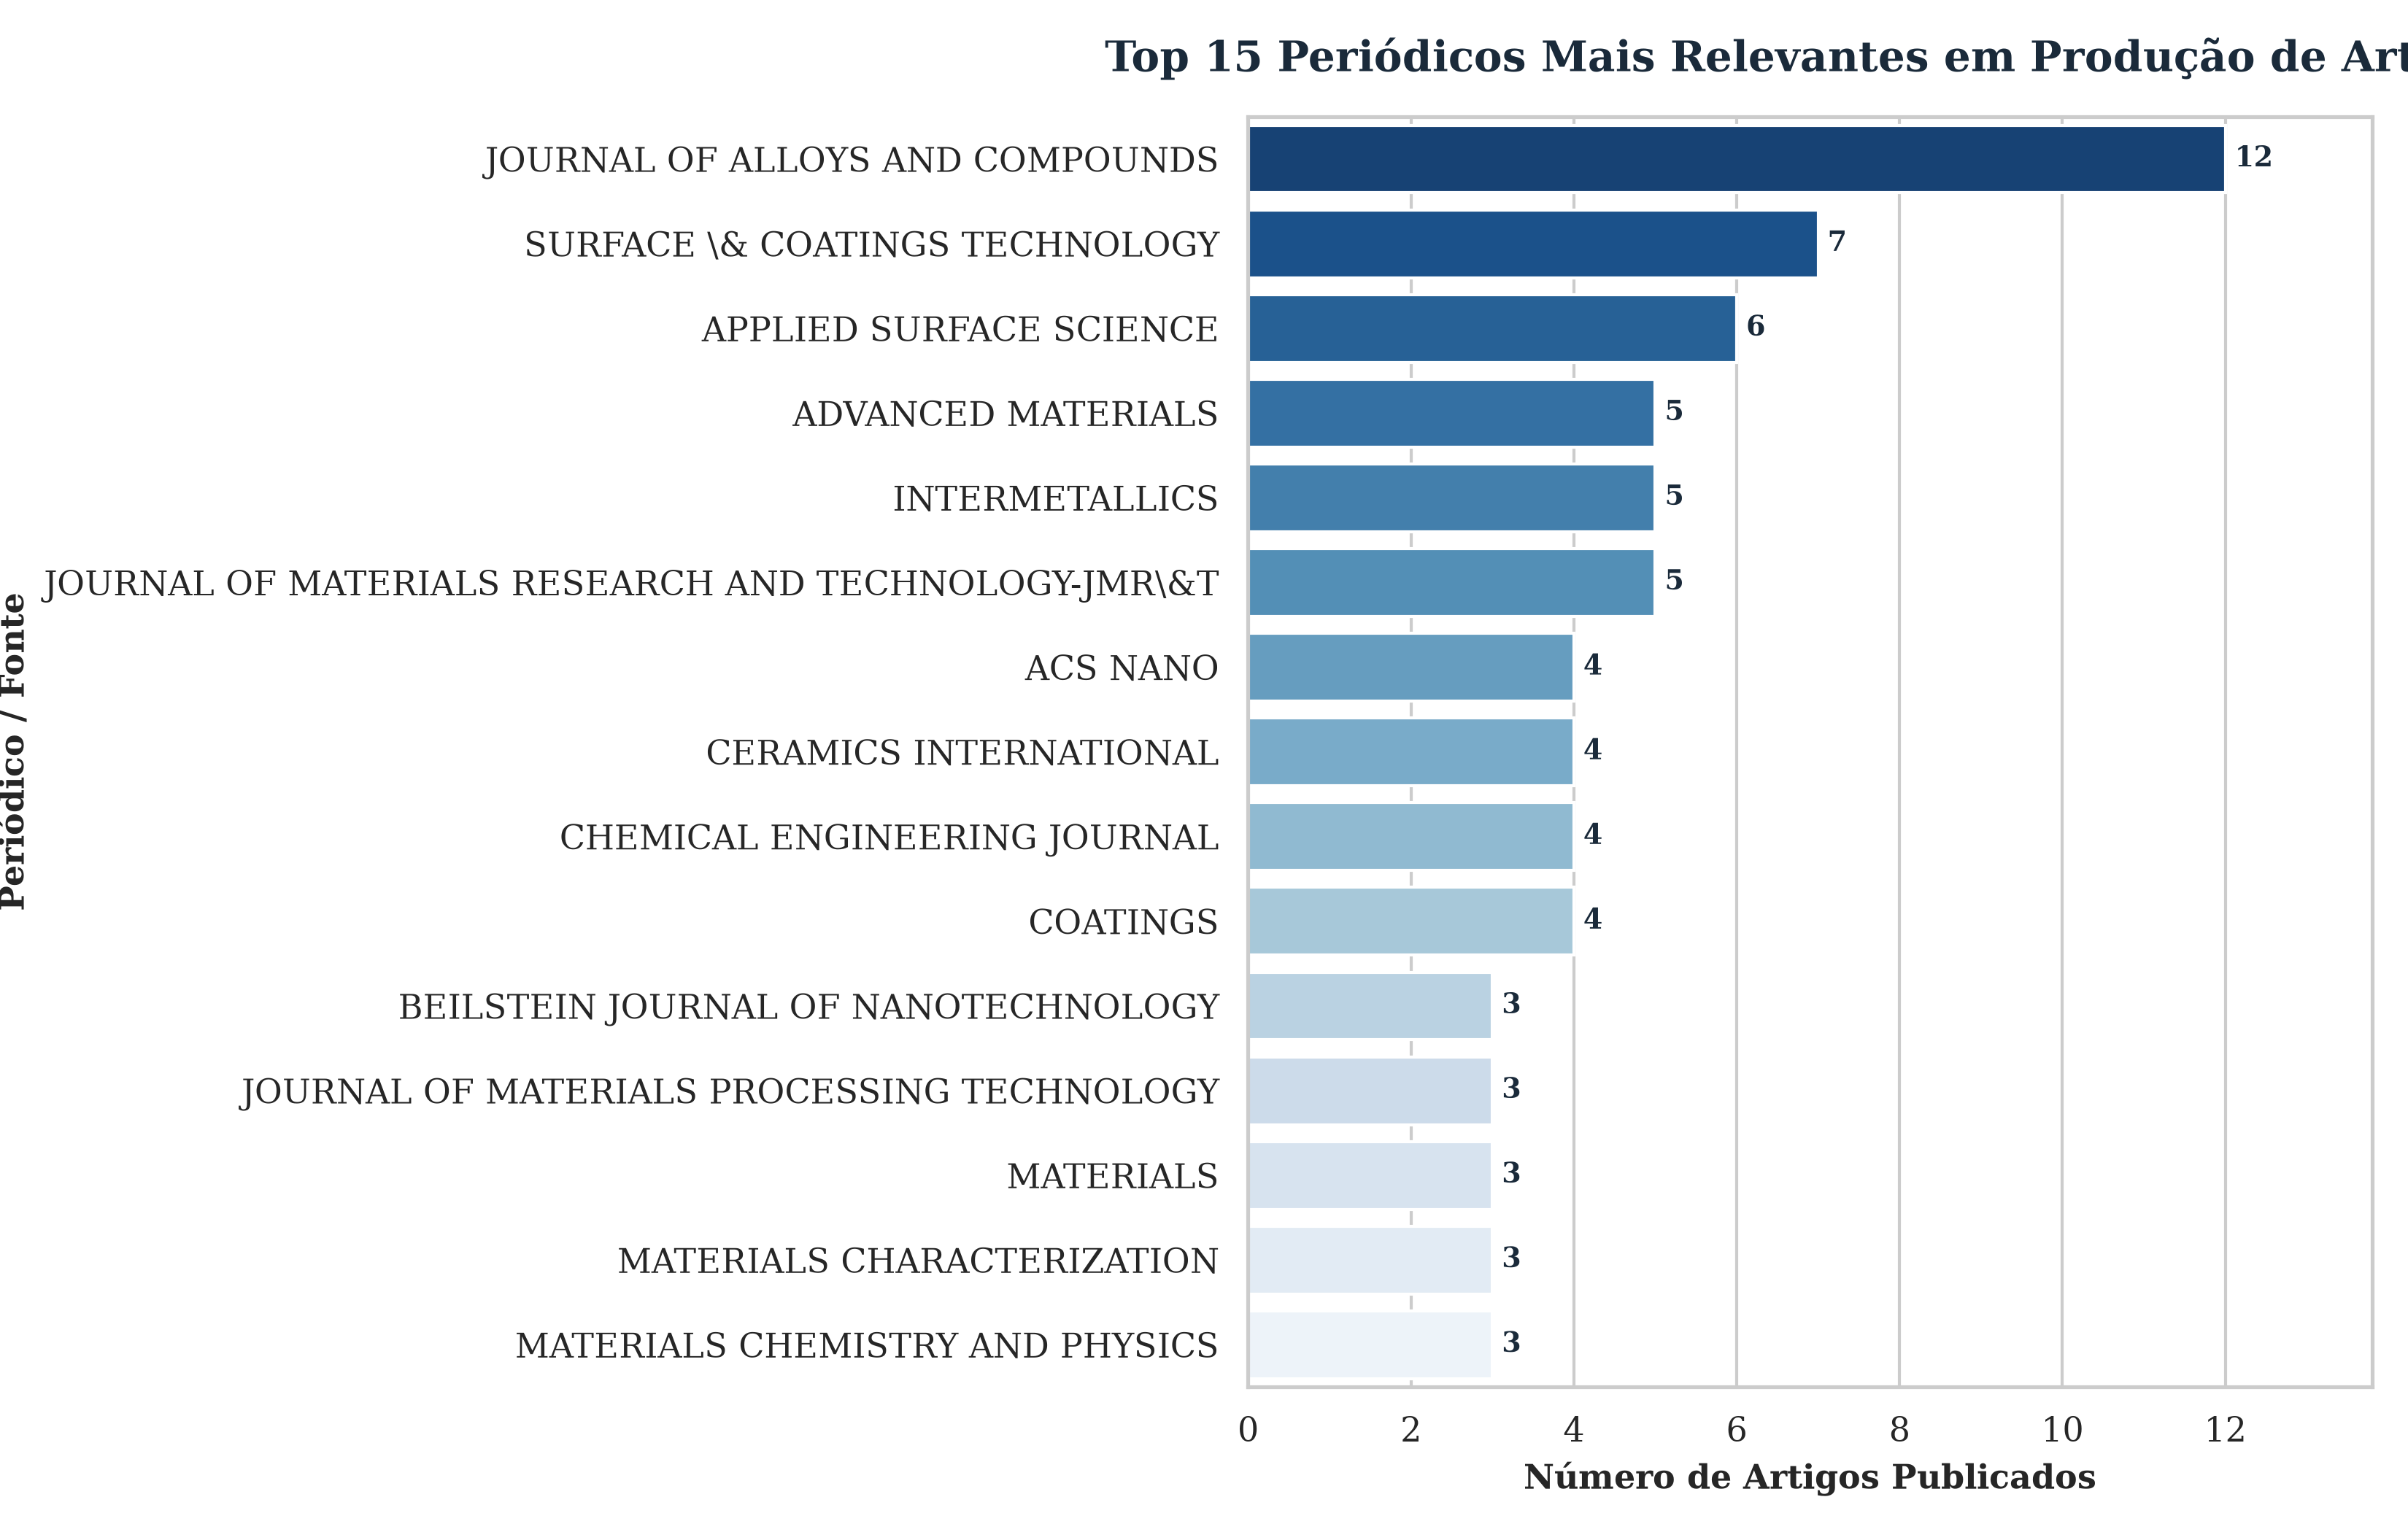
\includegraphics[width=0.85\textwidth]{figuras/most_relevant_sources.png}
\legend{Fonte: Elaborado pelos autores (2026), a partir de dados da \emph{Web of Science}.}
\end{figure}


Complementarmente, a Figura~\ref{fig:local_sources} ilustra as fontes mais citadas localmente (\emph{Local Cited Sources}), ou seja, os periódicos cujos artigos fundamentam teoricamente as pesquisas internas do corpus de 192 documentos. O \emph{Journal of Alloys and Compounds} lidera com 423 citações locais, seguido por \emph{Acta Materialia} (331 citações) e \emph{Nature Communications} (271 citações), reafirmando a convergência entre caracterização microestrutural avançada e resistência a solicitações extremas.

\begin{figure}[!htbp]
\centering
\caption{Fontes de publicação mais citadas no conjunto de referências internas do corpus.}\label{fig:local_sources}
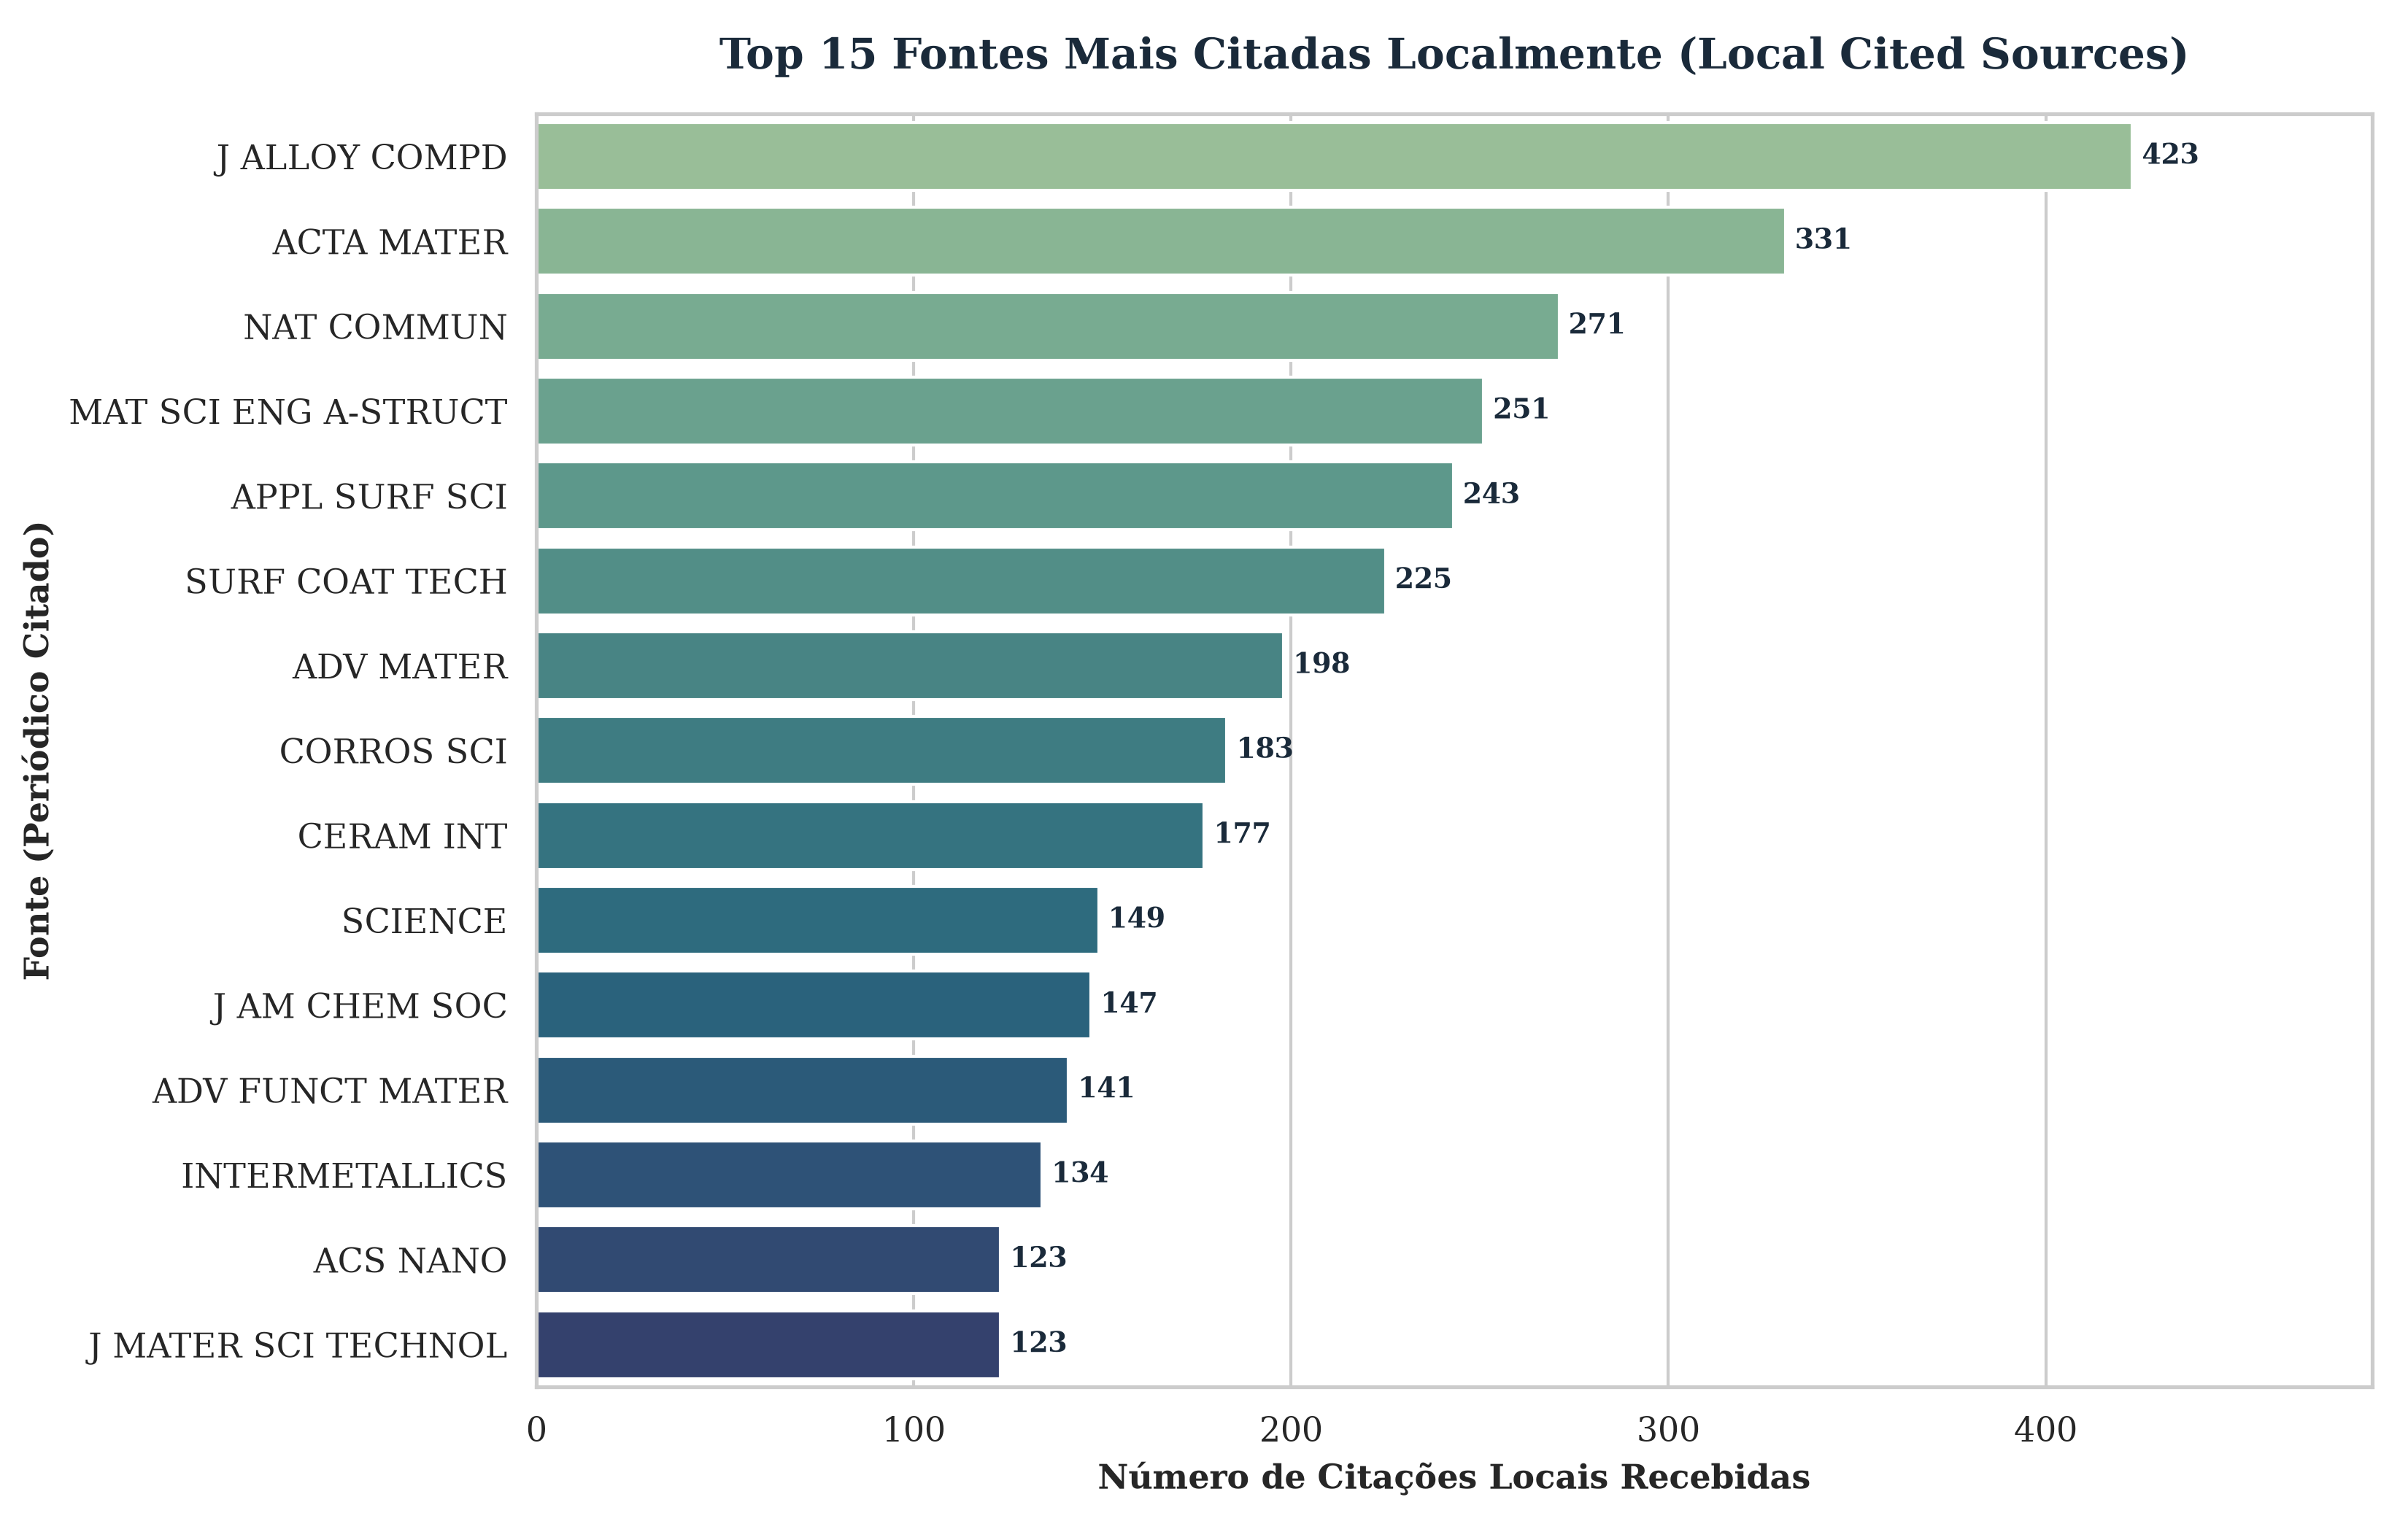
\includegraphics[width=0.85\textwidth]{figuras/most_local_cited_sources.png}
\legend{Fonte: Elaborado pelos autores (2026), a partir de dados da \emph{Web of Science}.}
\end{figure}

\subsection{Arquitetura Autoral, Institucional e Colaboração Geográfica}\label{arquitetura-autoral-institucional-e-colaboracao-geografica}

A análise de produtividade autoral no corpus atualizado (Figura~\ref{fig:relevant_authors} e Tabela~\ref{tab:authors_top10}) revela uma liderança marcante de centros de excelência em síntese de materiais e engenharia de superfícies. Destaca-se a forte atuação de pesquisadores da Alemanha (liderados por Stephan Barcikowski, Bilal Gökce, Lorenz Kienle e Christoph Rehbock) e de grupos internacionais de ponta em caracterização de materiais e fabricação aditiva na Ásia e América do Norte.

Sob a ótica do rigor cienciométrico, a interpretação da produtividade exige atenção crítica ao conhecido \textbf{efeito da homonímia} (\emph{Author Name Disambiguation} -- AND). Em bases de dados que indexam autores pela inicial e sobrenome, pesquisadores homônimos podem ser indevidamente agrupados. A verificação manual via identificadores persistentes (ORCID) e afiliações institucionais assegura a consistência das contribuições científicas identificadas neste mapeamento.

\begin{figure}[!htbp]
\centering
\caption{Os autores mais produtivos no corpus atualizado e auditado de 192 documentos.}\label{fig:relevant_authors}
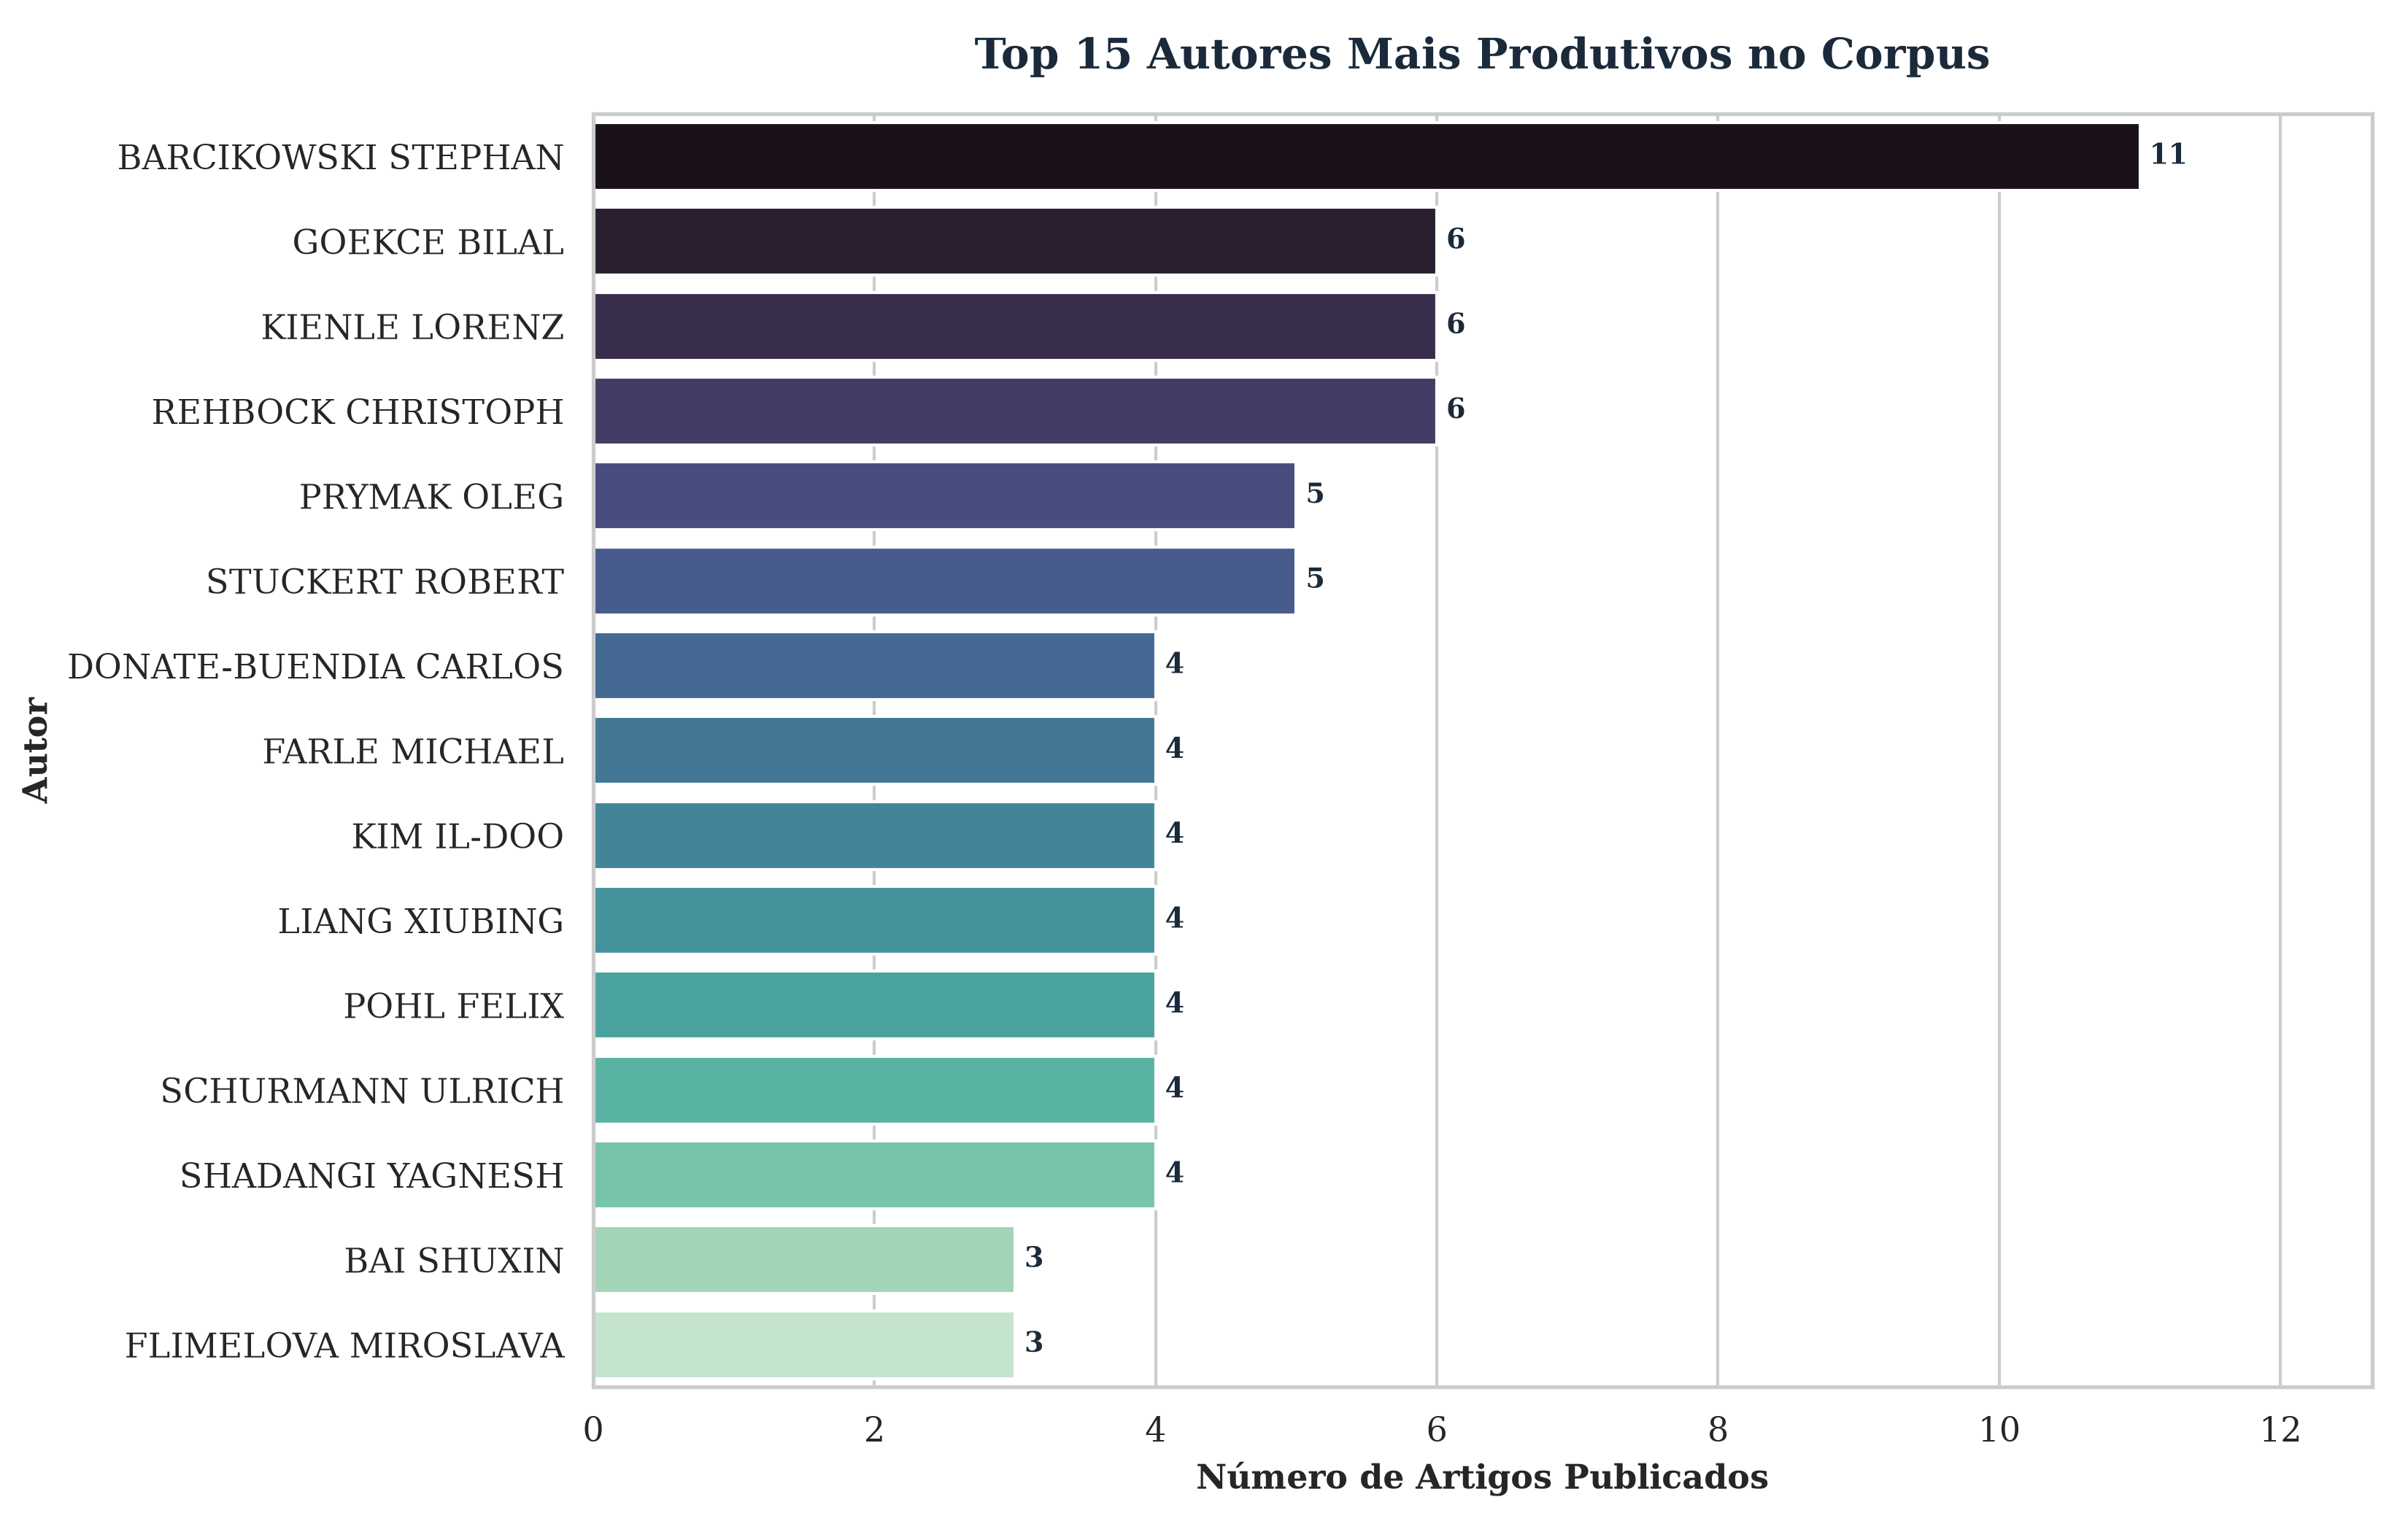
\includegraphics[width=0.85\textwidth]{figuras/most_relevant_authors.png}
\legend{Fonte: Elaborado pelos autores (2026), a partir de dados da \emph{Web of Science}.}
\end{figure}

\begin{table}[!htbp]
\centering
\caption{Os 10 Autores Mais Produtivos no Corpus e Principais Afiliações}\label{tab:authors_top10}
\small
\begin{tabularx}{\textwidth}{lc>{\raggedright\arraybackslash}X}
\toprule
\textbf{Autor} & \textbf{Artigos} & \textbf{Afiliação Institucional Dominante} \\
\midrule
BARCIKOWSKI S & 11 & University of Duisburg-Essen (Alemanha) \\
GOEKCE B & 6 & Univ. Wuppertal / Duisburg-Essen (Alemanha) \\
KIENLE L & 6 & University of Kiel (Alemanha) \\
REHBOCK C & 6 & University of Duisburg-Essen (Alemanha) \\
PRYMAK O & 5 & University of Duisburg-Essen (Alemanha) \\
STUCKERT R & 5 & University of Duisburg-Essen (Alemanha) \\
DONATE-BUENDIA C & 4 & Univ. Jaume I (Espanha) / Duisburg-Essen \\
FARLE M & 4 & University of Duisburg-Essen (Alemanha) \\
KIM ID & 4 & KAIST (Coreia do Sul) \\
LIANG XB & 4 & Academy of Armored Forces Engineering (China) \\
\bottomrule
\end{tabularx}
\legend{Fonte: Elaborado pelos autores (2026), com base em dados da \emph{Web of Science}.}
\end{table}

A distribuição das afiliações institucionais mais produtivas (Figura~\ref{fig:relevant_affiliations}) reforça esse ecossistema colaborativo. A \emph{University of Duisburg-Essen} (39 artigos) lidera o \emph{ranking} global com folga, seguida pela \emph{Shandong University} (16 artigos), \emph{University of Hyderabad} (12 artigos), \emph{Tianjin University of Technology and Education} (10 artigos) e \emph{Xi'an Jiaotong University} (10 artigos).

\begin{figure}[!htbp]
\centering
\caption{Afiliações institucionais mais produtivas no corpus de 192 documentos.}\label{fig:relevant_affiliations}
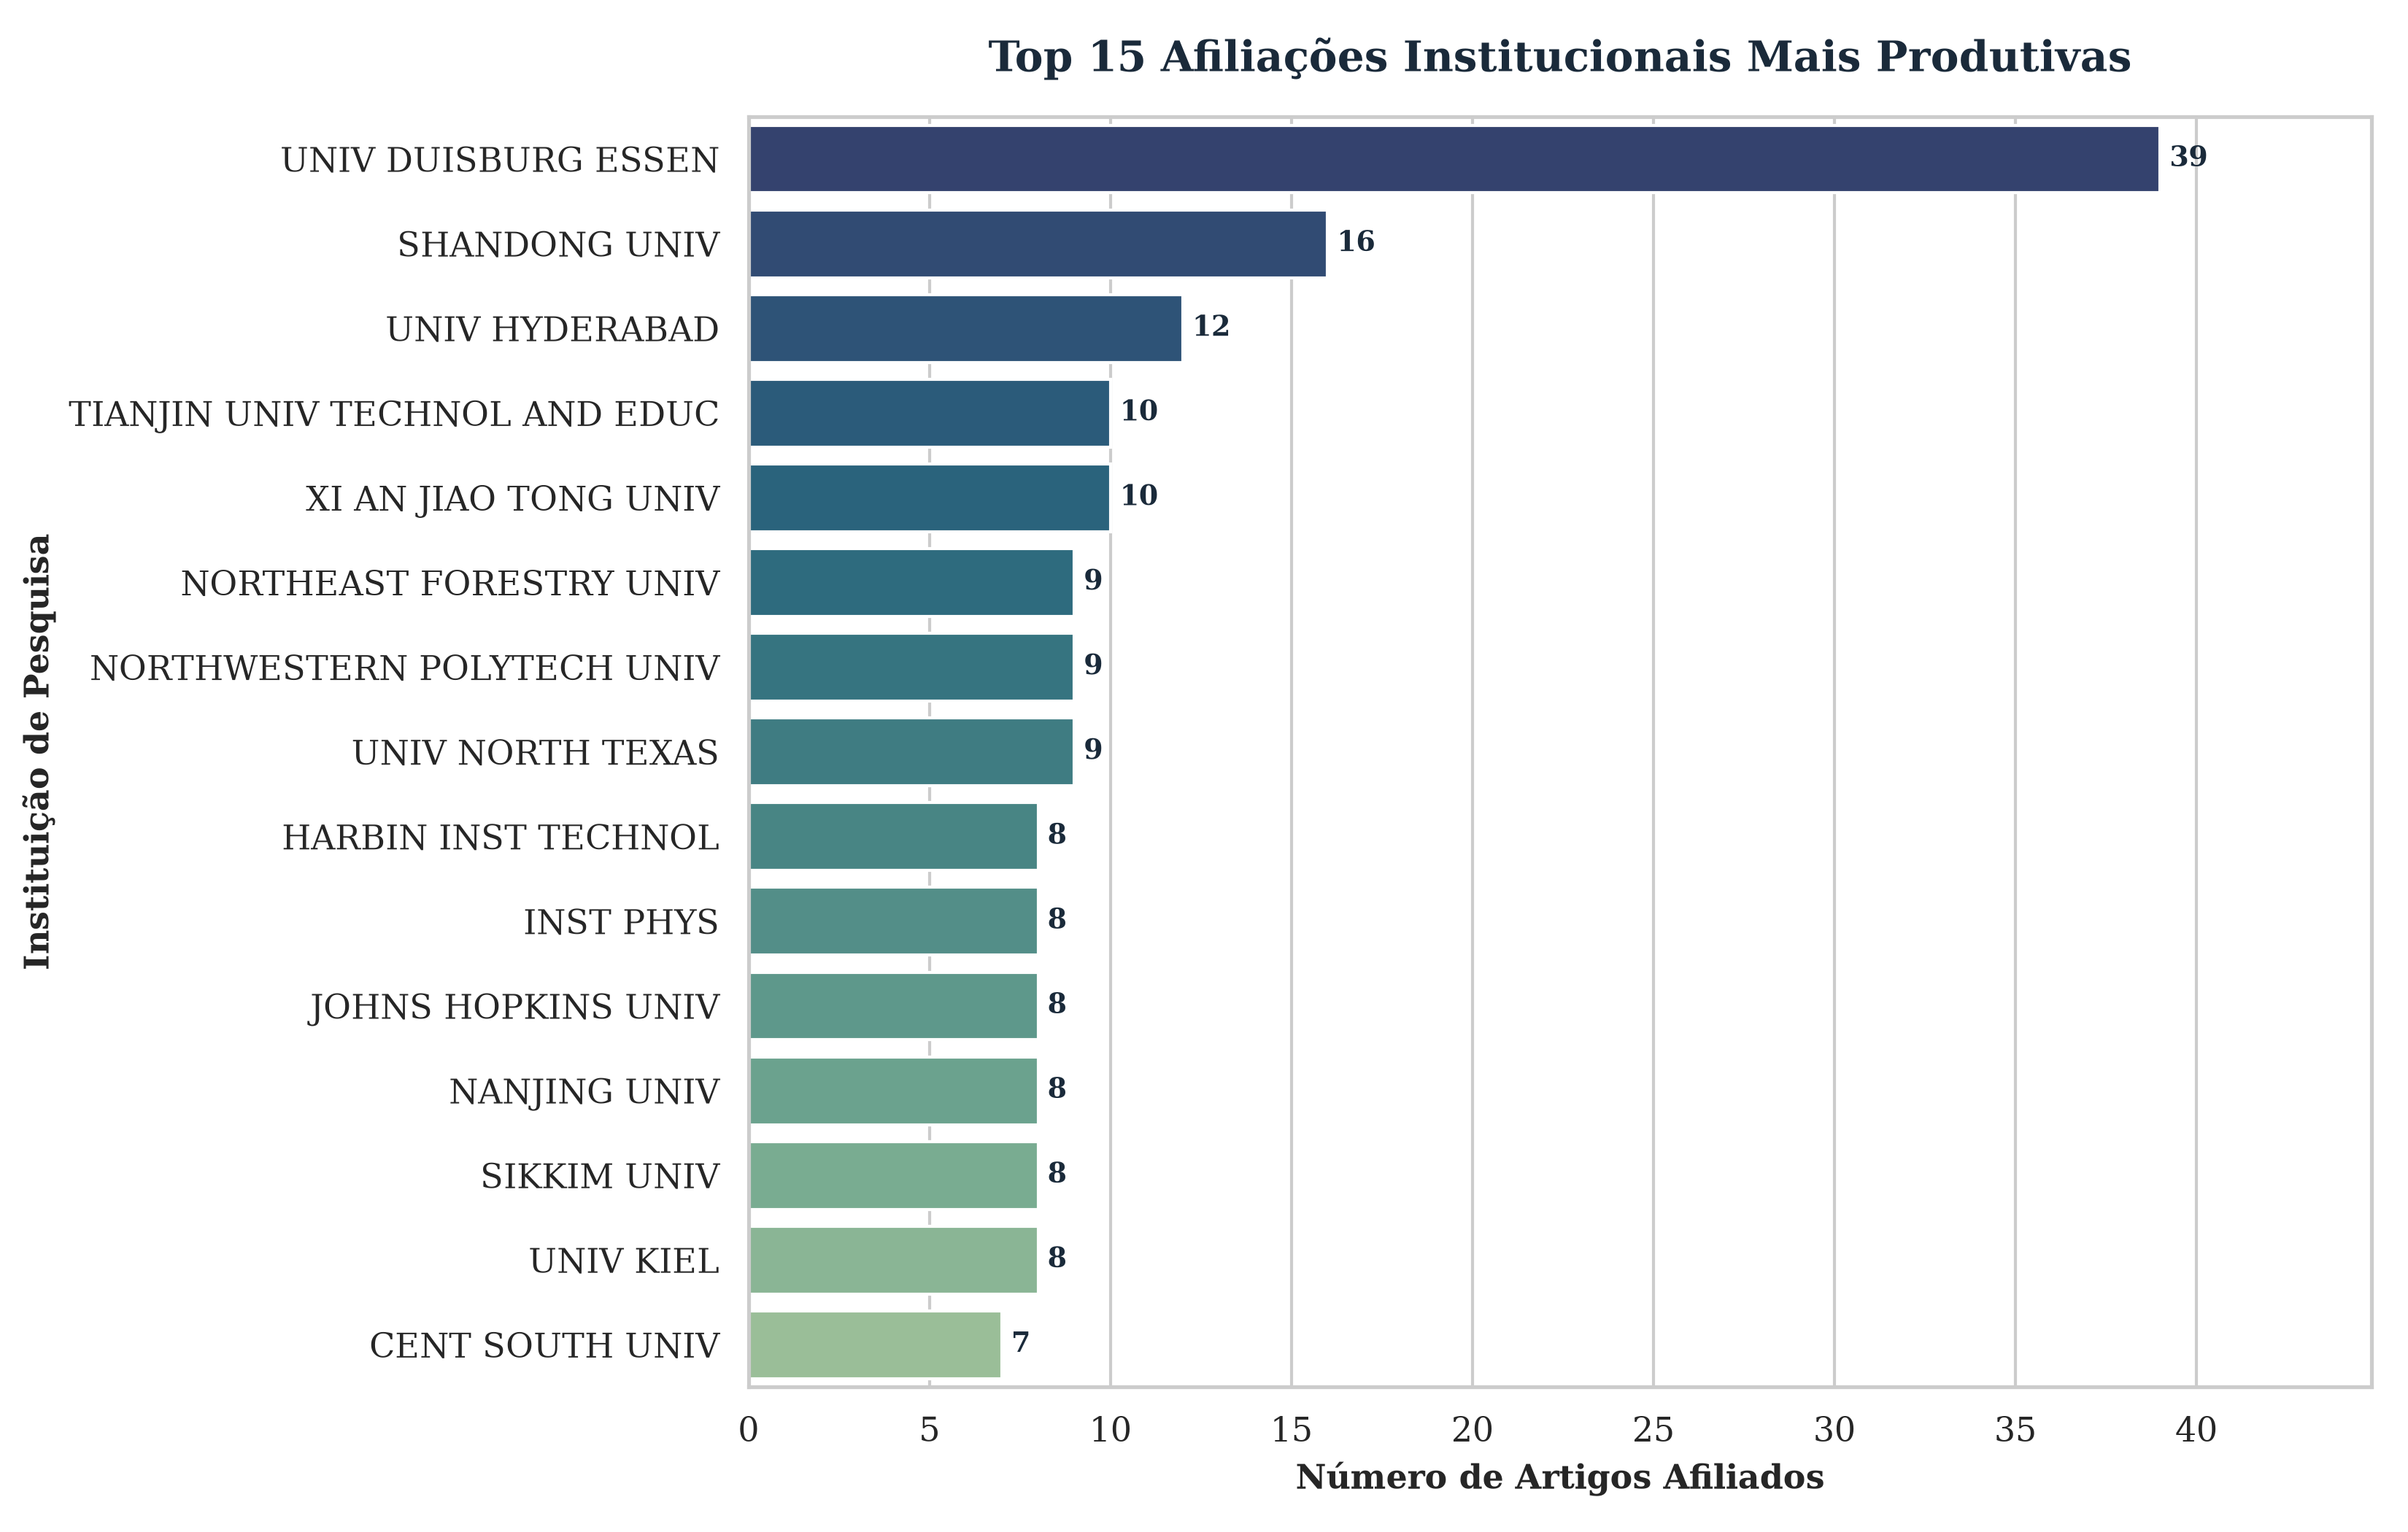
\includegraphics[width=0.85\textwidth]{figuras/most_relevant_affiliations.png}
\legend{Fonte: Elaborado pelos autores (2026), a partir de dados da \emph{Web of Science}.}
\end{figure}

A rede de colaboração internacional e cocitação, exposta na Figura~\ref{fig:collaboration_network}, demonstra agrupamentos fortemente conectados regionalmente, indicando a presença de consórcios nacionais e parcerias estratégicas de pesquisa impulsionando ligas refratárias.

\begin{figure}[!htbp]
\centering
\caption{Rede de cocitação e agrupamento intelectual construída via análise topológica (NetworkX), demonstrando centralidade e modularidade dos clusters no campo das RHEAs.}\label{fig:collaboration_network}
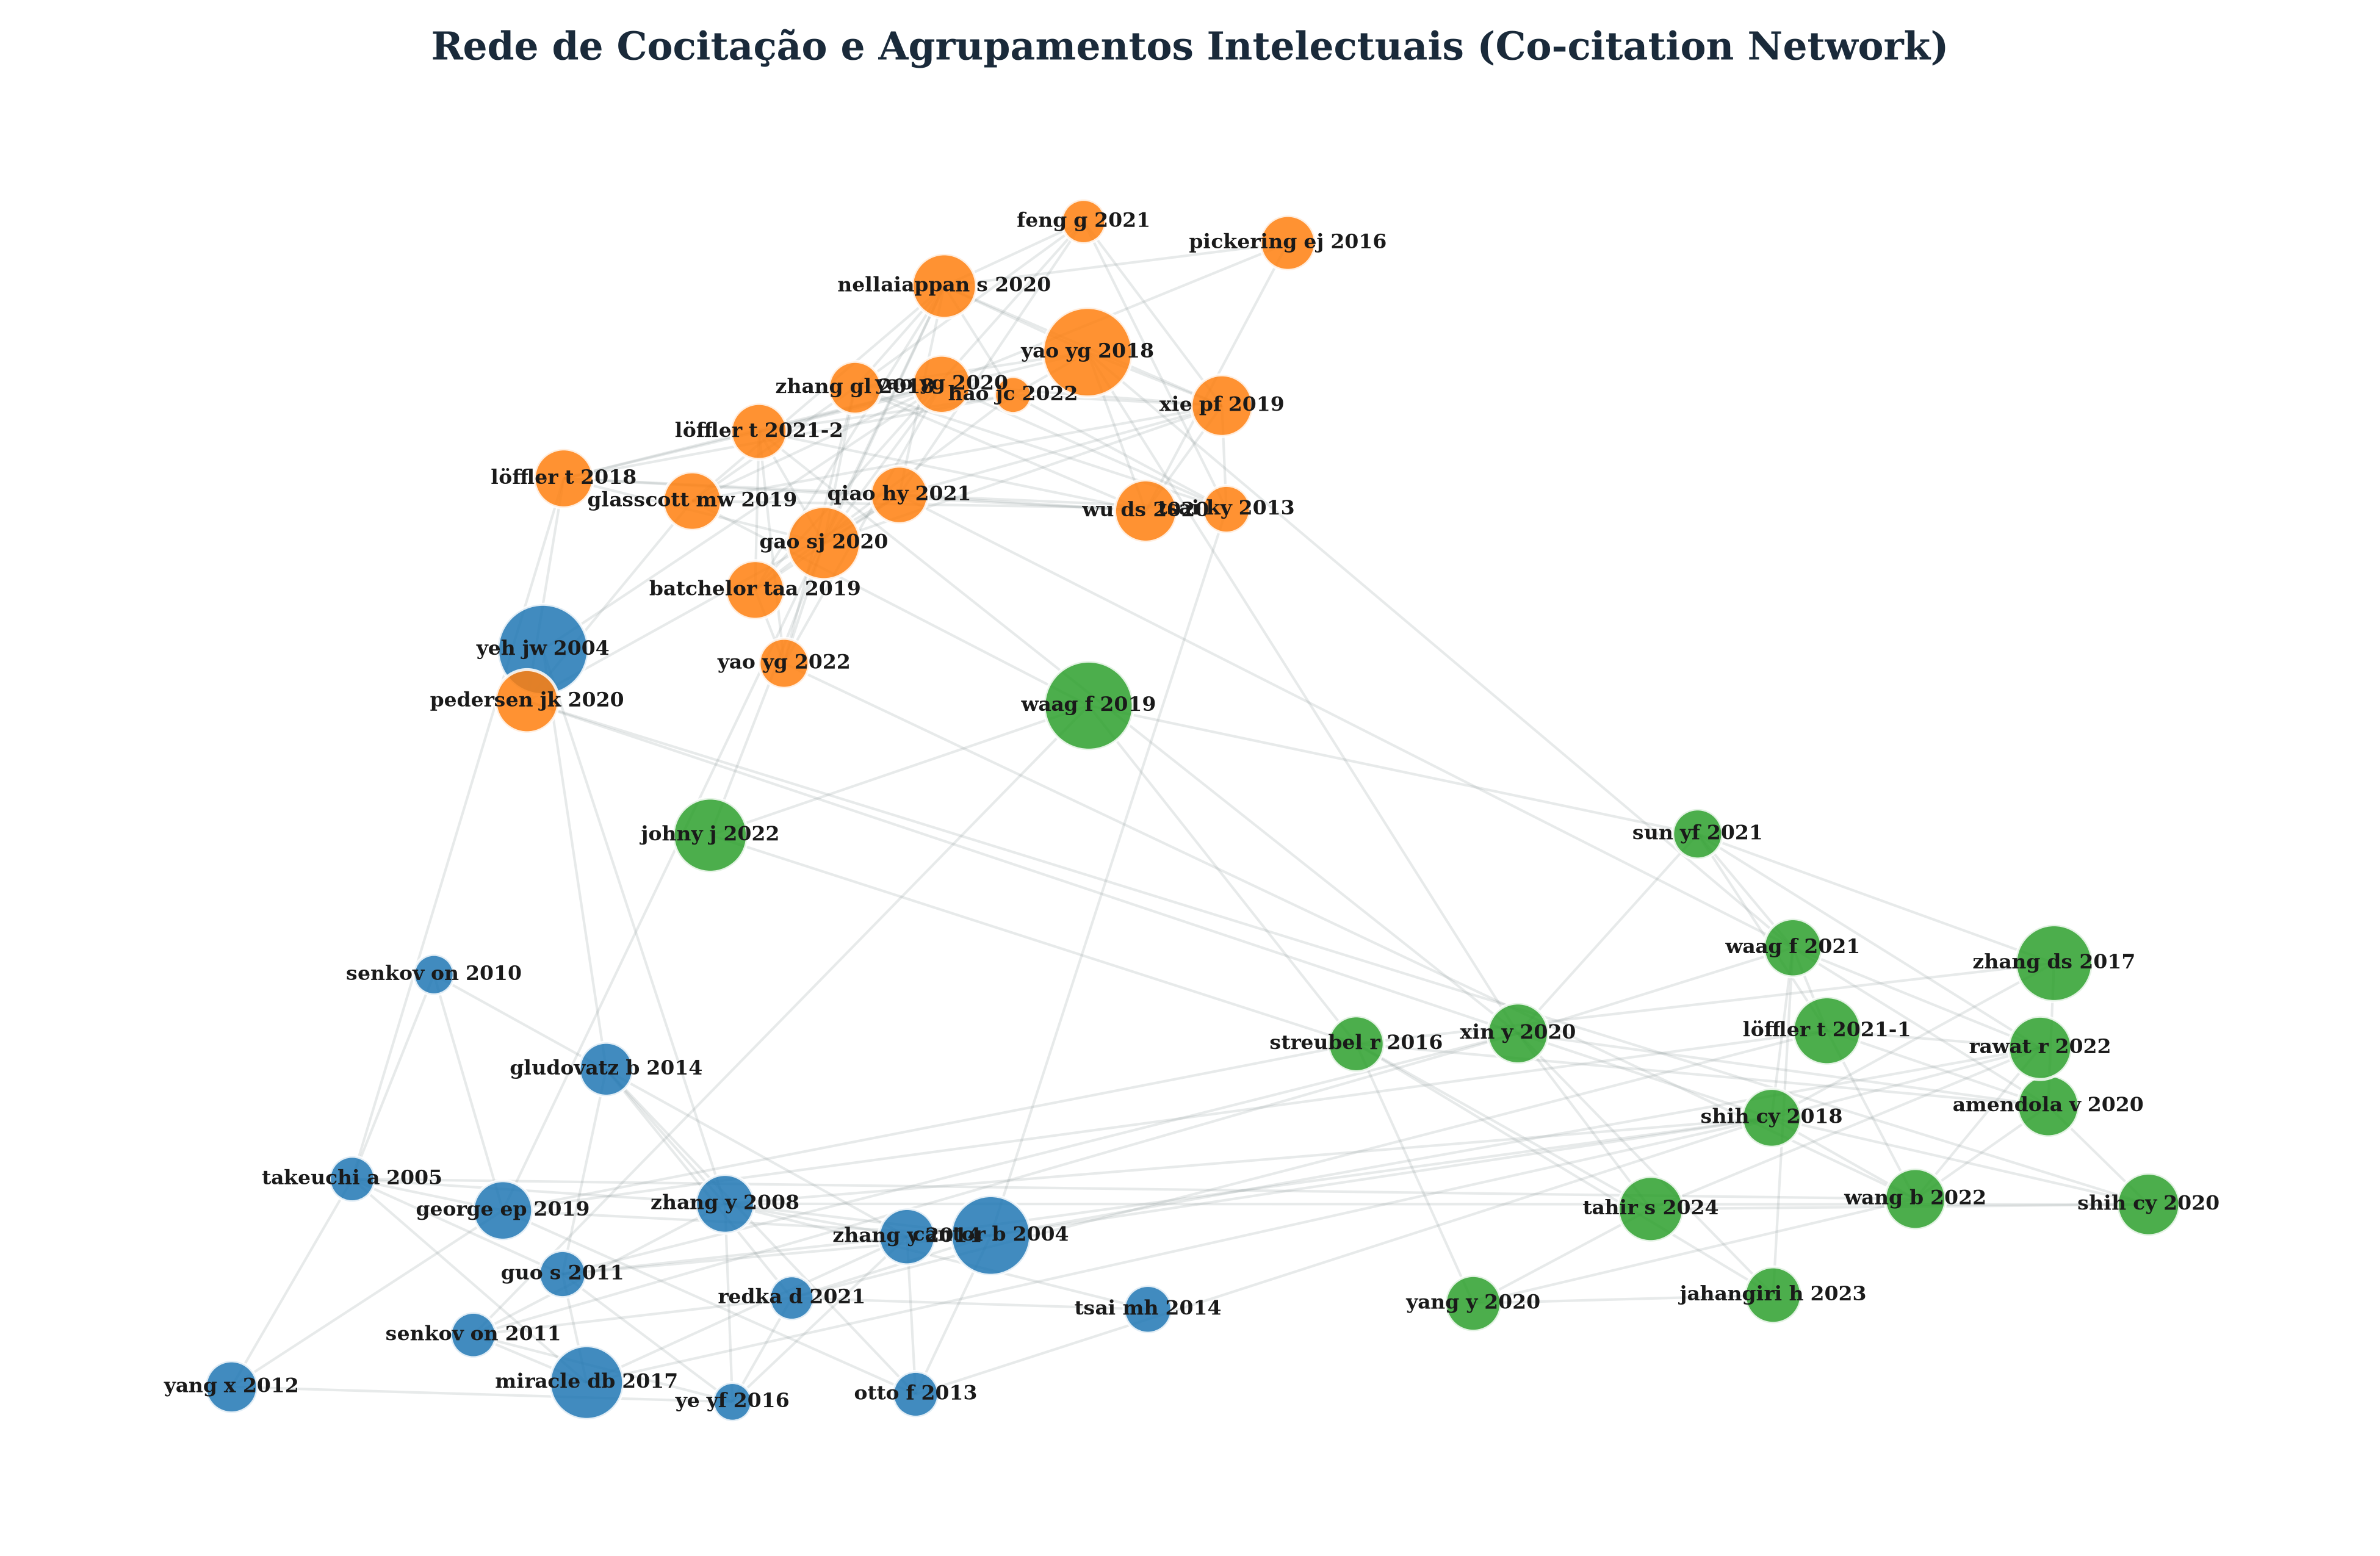
\includegraphics[width=0.85\textwidth]{figuras/cocit_network.png}
\legend{Fonte: Elaborado pelos autores (2026), a partir de dados da \emph{Web of Science}.}
\end{figure}

\subsection{Artigos Mais Citados Global e Localmente}\label{artigos-mais-citados-global-e-localmente}

O impacto das publicações no ecossistema científico global é apresentado na Figura~\ref{fig:global_cited} e sumarizado na Tabela~\ref{tab:top_glob_docs}. O estudo de Peters et al. (2024), publicado na \emph{Nature Communications}, desponta como o artigo mais citado globalmente (462 citações e notável taxa de 154 citações por ano), destacando-se na fronteira de design de materiais para aplicações hipersônicas. É seguido por Wang B. et al. (2022) na \emph{Nature Synthesis} (302 citações; 60,40 cit./ano) e por Waag et al. (2019) na \emph{RSC Advances} (242 citações).

\begin{figure}[!htbp]
\centering
\caption{Os artigos mais citados globalmente dentro do conjunto de dados.}\label{fig:global_cited}
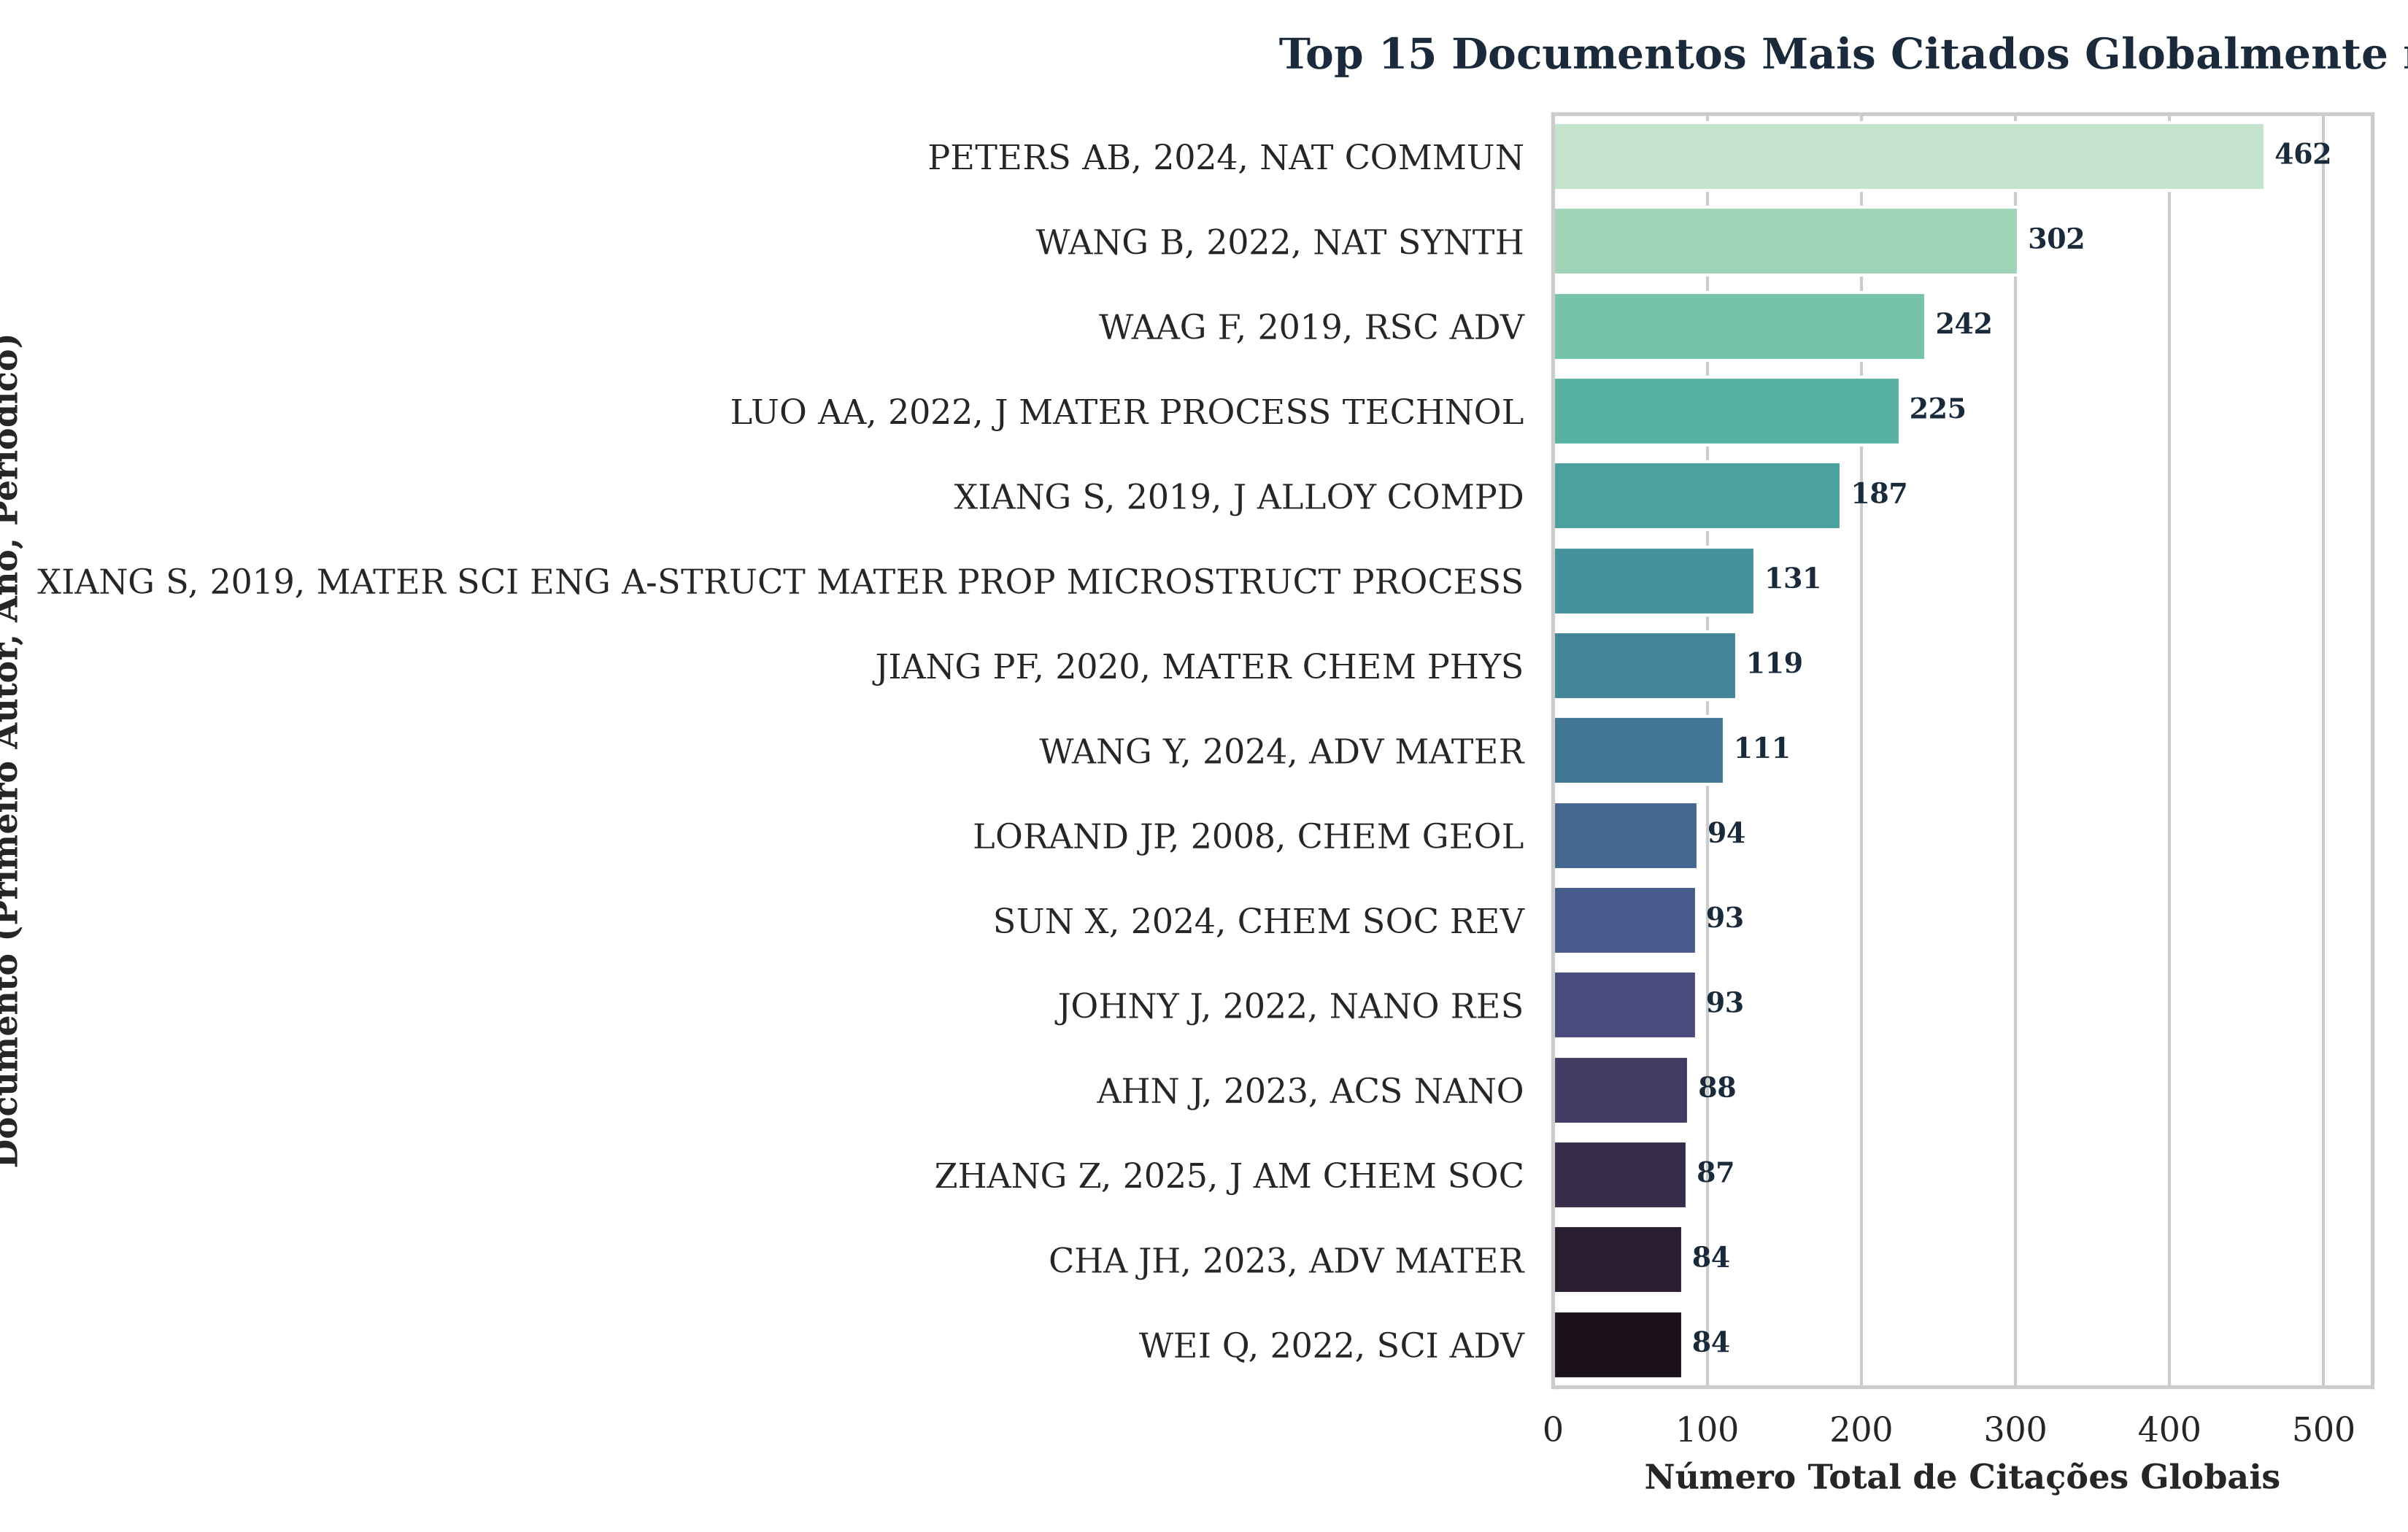
\includegraphics[width=0.85\textwidth]{figuras/most_global_cited_documents.png}
\legend{Fonte: Elaborado pelos autores (2026), a partir de dados da \emph{Web of Science}.}
\end{figure}

\begin{table}[!htbp]
\centering
\caption{Os 10 Artigos Mais Citados Globalmente no Corpus Atualizado}\label{tab:top_glob_docs}
\footnotesize
\begin{tabularx}{\textwidth}{l>{\raggedright\arraybackslash}Xlcc}
\toprule
\textbf{Autor e Ano} & \textbf{Título do Estudo} & \textbf{Periódico} & \textbf{Cit.} & \textbf{Cit./Ano} \\
\midrule
PETERS AB (2024) & Materials design for hypersonics & \emph{Nat. Commun.} & 462 & 154,00 \\
WANG B (2022) & General synthesis of HEA and ceramic nanoparticles & \emph{Nat. Synth.} & 302 & 60,40 \\
WAAG F (2019) & Kinetically-controlled laser-synthesis of colloidal HEAs & \emph{RSC Adv.} & 242 & 30,20 \\
LUO AA (2022) & Alloy development and process innovations for light metals & \emph{J. Mater. Process. Technol.} & 225 & 45,00 \\
XIANG S (2019) & Microstructures and mechanical properties of CrMnFeCoNi & \emph{J. Alloys Compd.} & 187 & 23,40 \\
XIANG S (2019) & Effects of process parameters on tensile properties of LMD & \emph{Mater. Sci. Eng. A} & 131 & 16,40 \\
JIANG PF (2020) & Fabrication and wear behavior of TiC reinforced HEA coatings & \emph{Mater. Chem. Phys.} & 119 & 17,00 \\
WANG Y (2024) & Self-Encapsulation of HEA Nanoparticles in Wood & \emph{Adv. Mater.} & 111 & 37,00 \\
LORAND JP (2008) & Abundance and distribution of PGE in orogenic lherzolites & \emph{Chem. Geol.} & 94 & 4,90 \\
SUN X (2024) & Synthesis of metallic high-entropy alloy nanoparticles & \emph{Chem. Soc. Rev.} & 93 & 31,00 \\
\bottomrule
\end{tabularx}
\legend{Fonte: Elaborado pelos autores (2026), com base em dados da \emph{Web of Science}.}
\end{table}

\begin{figure}[!htbp]
\centering
\caption{Obras fundamentais mais citadas localmente pelo corpus de 192 documentos.}\label{fig:local_cited}
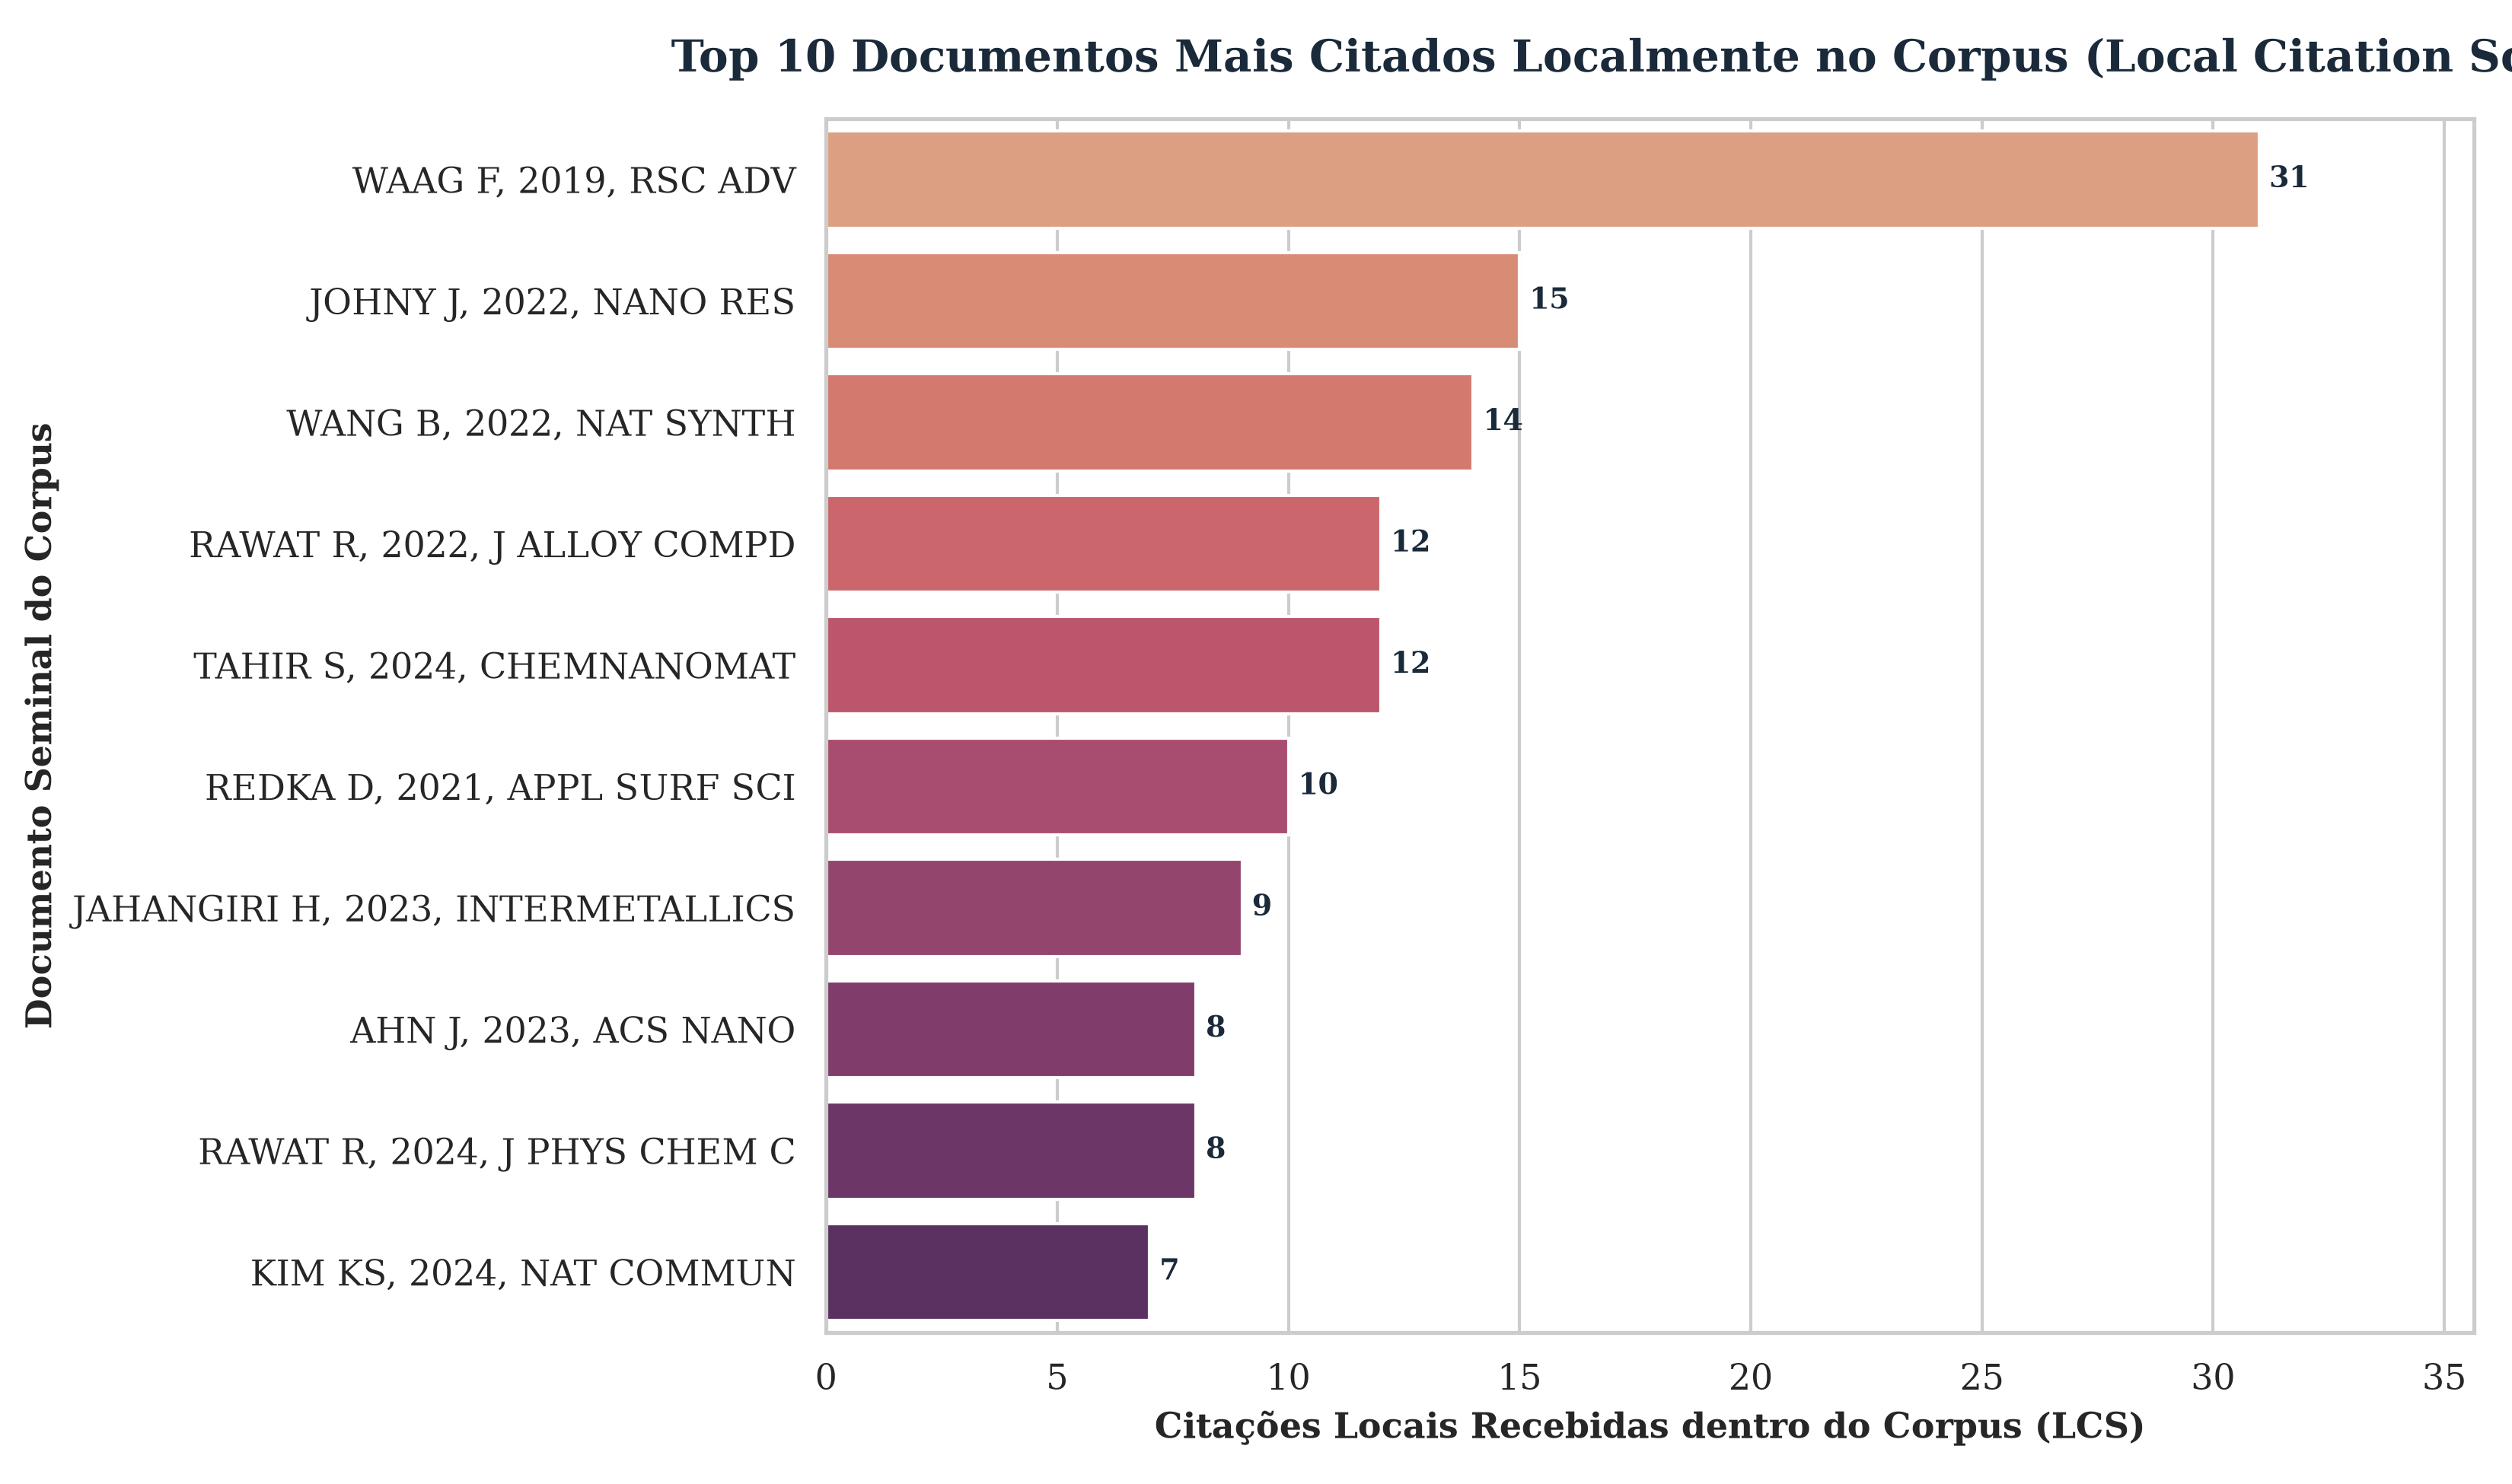
\includegraphics[width=0.85\textwidth]{figuras/most_local_cited_documents.png}
\legend{Fonte: Elaborado pelos autores (2026), a partir de dados da \emph{Web of Science}.}
\end{figure}

\subsection{A Espinha Dorsal Intelectual: De Yeh e Cantor às Ligas Refratárias}\label{a-espinha-dorsal-intelectual-de-yeh-e-cantor-as-ligas-refratarias}

A análise das citações locais na Figura~\ref{fig:local_cited} e nas referências históricas do corpus demonstra a dependência teórico-conceitual do campo em relação a pilares seminais. De um lado, as investigações de Jien-Wei Yeh et al. (2004) e Brian Cantor et al. (2004) romperam com o paradigma clássico do elemento solvente único, formalizando a entropia configuracional ($\Delta S_{\text{conf}} \ge 1{,}5R$) para estabilizar soluções sólidas desordenadas simples (BCC, FCC, HCP) e introduzindo a clássica liga CoCrFeMnNi. De outro lado, Oleg N. Senkov et al. (2010, 2011, 2012, 2018) transpuseram esses princípios termodinâmicos para elementos refratários de ultra-alto ponto de fusão (W, Ta, Mo, Nb, V, Ti, Zr e Hf), demonstrando que sistemas equiatômicos como WNbMoTa e WNbMoTaV retêm limites de escoamento superiores a 400 MPa a 1600 \textdegree{}C, patamar inatingível para superligas à base de níquel.

\subsection{Análise de Palavras-chave e Evolução Temática}\label{sec:analise_palavras_chave}

A análise de palavras-chave permite identificar os principais eixos temáticos e as frentes emergentes da literatura sobre ligas de alta entropia para condições extremas. A partir da frequência e coocorrência dos termos no corpus (Figura~\ref{fig:wordcloud}), a produção científica articula-se em três eixos interdependentes. O primeiro eixo abrange a \textbf{microestrutura e propriedades mecânicas}, com ênfase na estabilização de fases e nos mecanismos de endurecimento (\emph{microstructure}, \emph{yield strength}, \emph{mechanical properties}) para sustentar solicitações mecânicas acima de 1200 \textdegree{}C. O segundo eixo concentra-se na \textbf{resistência ambiental e oxidação}, investigando a degradação sob alta temperatura (\emph{oxidation}, \emph{high-temperature oxidation}) e a inibição da oxidação catastrófica (\emph{pest oxidation}) intrínseca a elementos refratários voláteis. O terceiro eixo focaliza o \textbf{processamento e revestimentos protetores}, impulsionando o desenvolvimento de barreiras térmicas (\emph{coatings}), rotas de metalurgia do pó e manufatura aditiva para integração em componentes aeroespaciais.

\begin{figure}[!htbp]
\centering
\caption{Nuvem de palavras-chave evidenciando os termos de maior frequência no corpus.}\label{fig:wordcloud}
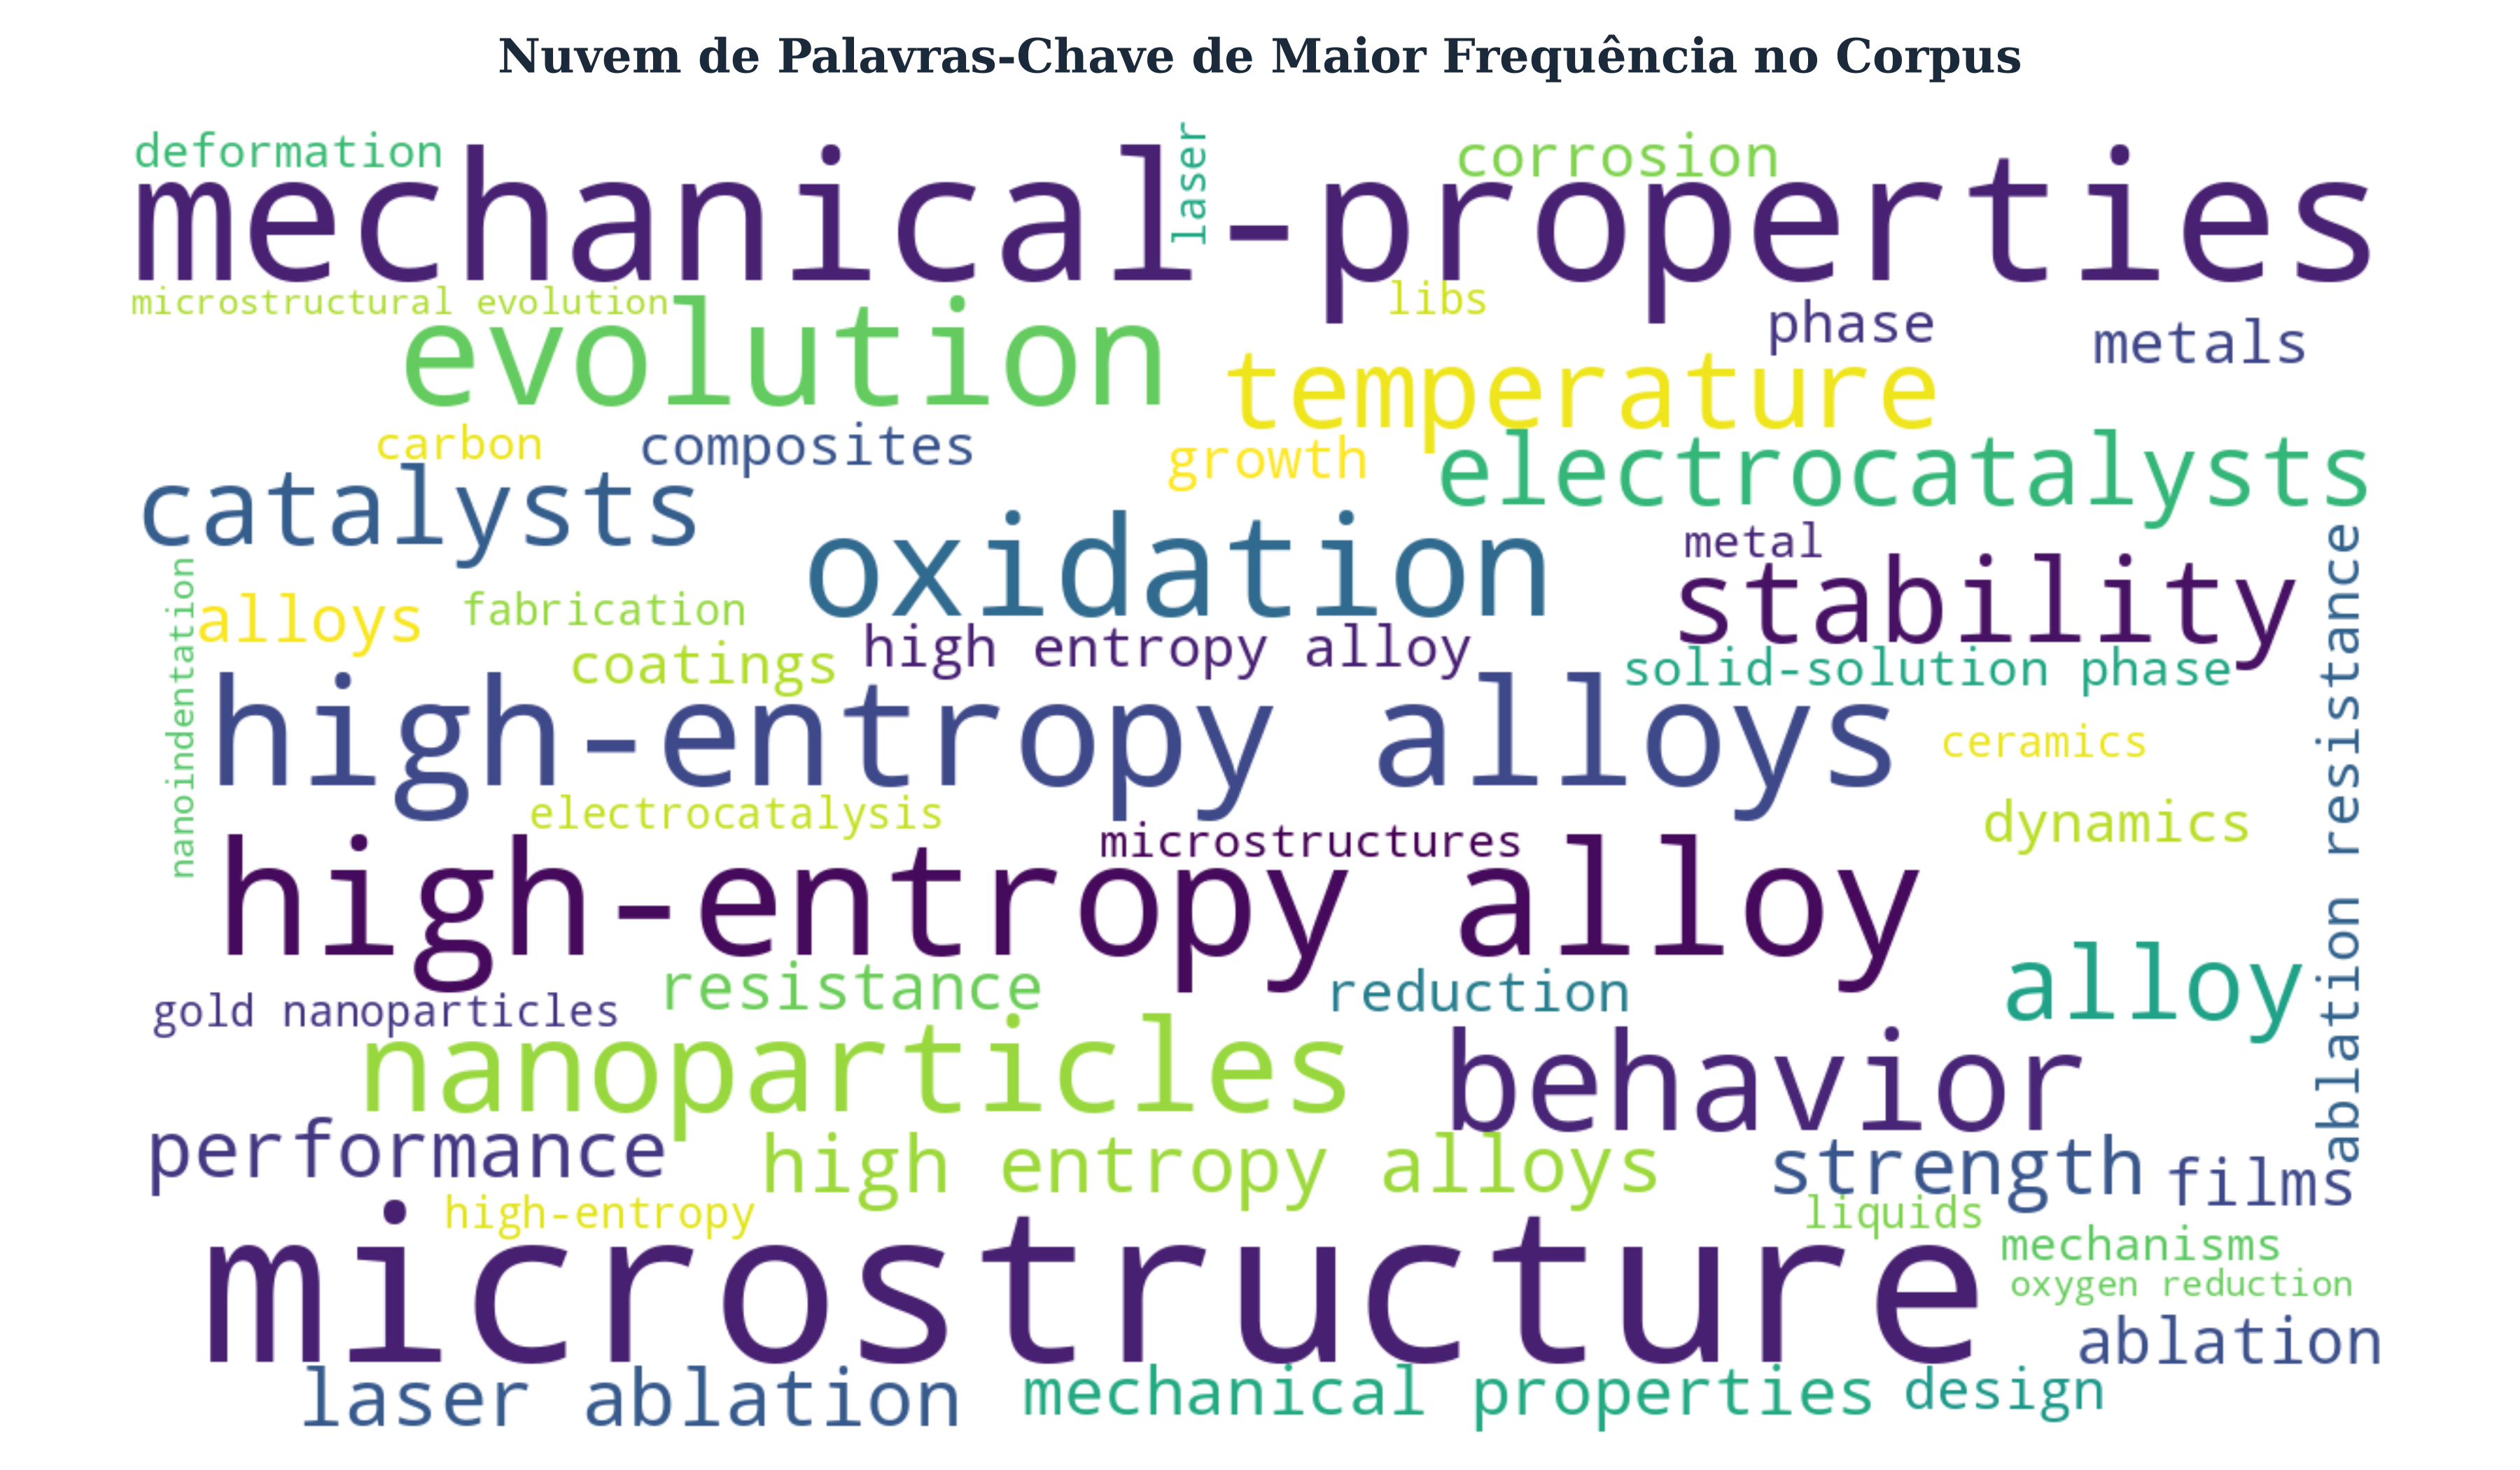
\includegraphics[width=0.85\textwidth]{figuras/wordcloud.png}
\legend{Fonte: Elaborado pelos autores (2026), a partir de dados da \emph{Web of Science}.}
\end{figure}

\begin{figure}[!htbp]
\centering
\caption{Evolução temporal das palavras-chave e tópicos de pesquisa no período 2013--2026.}\label{fig:trend_topics}
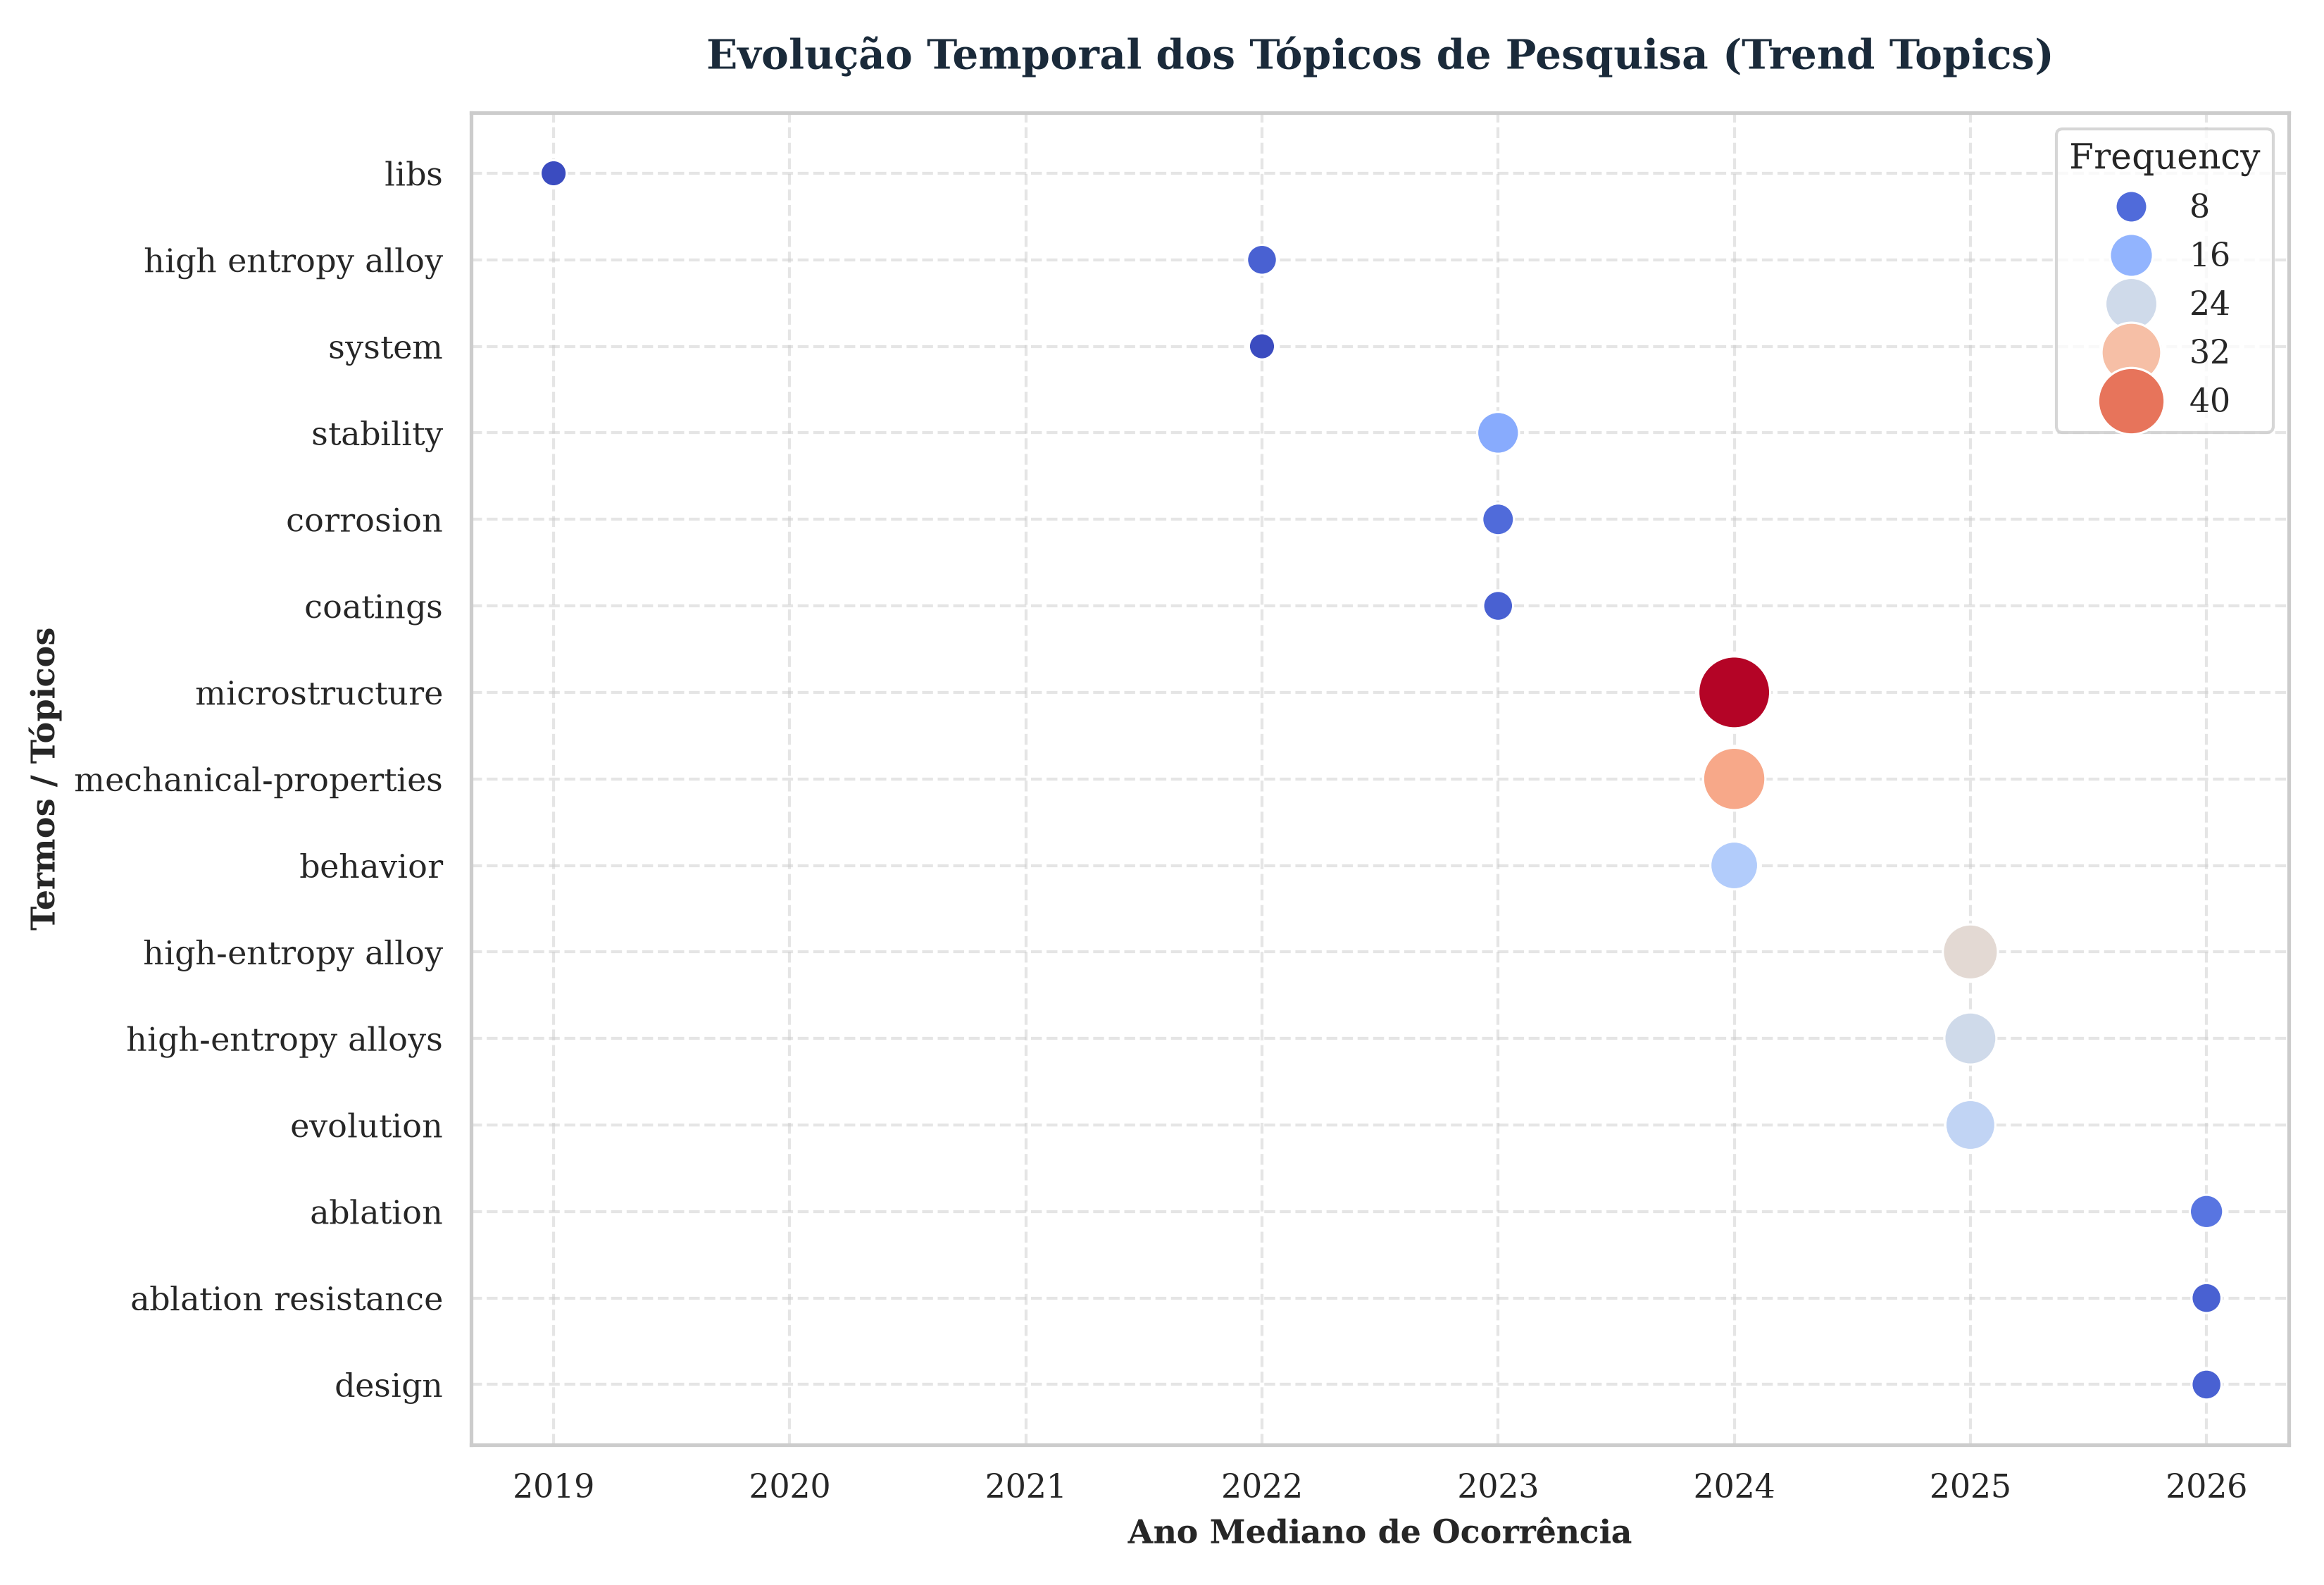
\includegraphics[width=0.85\textwidth]{figuras/trend_topics.png}
\legend{Fonte: Elaborado pelos autores (2026), a partir de dados da \emph{Web of Science}.}
\end{figure}

A análise temporal dos tópicos de pesquisa (Figura~\ref{fig:trend_topics}) evidencia a maturidade gradual da área. Nos primeiros anos (2013--2018), as publicações concentravam-se na caracterização básica de microestrutura, dureza e comportamento em compressão. A partir de 2019, observa-se uma transição nítida em direção à engenharia de ligas aplicadas, destacando-se temas como cinética de oxidação em temperaturas ultra-altas, revestimentos protetores contra ablação e, mais recentemente (2023--2026), o emprego de manufatura aditiva e ferramentas computacionais (CALPHAD e aprendizado de máquina) para aceleração do design composicional.

\subsection{Redes de Cocitação e Acoplamento Bibliográfico}\label{redes-de-cocitacao-e-acoplamento-bibliografico}

A investigação relacional profunda (\emph{Co-citation Network}) confirma a força gravitacional dos fundadores da área. A análise visual de cocitação (referências antigas frequentemente citadas de forma conjunta) atesta que os estudos seminais de Yeh e Cantor (2004) constituem um agrupamento central indissociável dos trabalhos basilares de Senkov (2010), comprovando que a academia percebe as ligas refratárias (RHEAs) como uma extensão ininterrupta e direta do marco termodinâmico de 2004. Por sua vez, o acoplamento bibliográfico (\emph{Bibliographic Coupling}), que agrupa as publicações atuais do corpus que compartilham o mesmo referencial, revela as atuais ``ilhas'' de pesquisa. Identifica-se uma frente focada agressivamente na mitigação de corrosão por meio de \emph{coatings} funcionais protetores e uma frente paralela, frequentemente oriunda do cenário europeu, baseada na predição exaustiva de estabilidade de fases por meio do método CALPHAD.



\subsection{Rede de Coocorrência Institucional e Geopolítica}\label{rede-de-coocorrencia-institucional-e-geopolitica}

O exame das macro-colaborações institucionais delineia a geopolítica da tecnologia de materiais. Enquanto os grafos de colaboração país-a-país indicam a China como a maior produtora em volume bruto, observam-se padrões frequentemente endógenos, onde instituições chinesas colaboram de forma massiva, porém domesticamente (como as conexões fortes entre HIT e Taiyuan). Em contrapartida, polos situados na Alemanha, nos Estados Unidos e na Inglaterra exibem altíssimos níveis de centralidade de intermediação (\emph{betweenness centrality}), operando como os nós conectores essenciais que distribuem o conhecimento ao redor do globo, tecendo redes complexas de transferência e validação de tecnologias para resistência termomecânica.

\subsection{Perspectivas Futuras: Aprendizado de Máquina e Intersticiais}\label{perspectivas-futuras-aprendizado-de-maquina-e-intersticiais}

Os desenvolvimentos recentes registrados na parcela final do corpus (2024--2026) apontam para metodologias emergentes, como a \textbf{Simbiose Machine Learning -- CALPHAD}, acelerando a previsão composicional termodinâmica em bancos de dados ab initio. Em suma, a expansão do corpus bibliométrico comprova que as Ligas de Alta Entropia Refratárias se consolidaram como a plataforma de materiais estruturais definitiva do século XXI.

\section{Microestrutura e Propriedades Mecânicas em Ligas de Alta Entropia Hipersónicas}\label{sec:microestrutura_propriedades_hea}

As Ligas de Alta Entropia (HEAs) e as Ligas Refratárias de Alta Entropia (RHEAs) são essenciais para viabilizar veículos hipersónicos ($M > 5$). Para que os componentes estruturais resistam a essas condições operacionais extremas, é necessário um controle rigoroso da relação entre a composição química, a estrutura interna (microestrutura) e o desempenho mecânico.

\subsection{A Microestrutura como Elo de Desempenho}\label{subsec:microestrutura_elo_desempenho}

O ambiente hipersónico impõe aos materiais choques térmicos brutais, com gradientes térmicos variando de $-170~^\circ\mathrm{C}$ a mais de $2000~^\circ\mathrm{C}$ em distâncias milimétricas, associados a pressões estagnadas e fluxos de plasma altamente reativos. Nesse regime extremo, a integridade estrutural é ditada pela arquitetura microestrutural subjacente. Enquanto matrizes cúbicas de corpo centrado (BCC) mantêm patamares mecânicos expressivos entre $1000~^\circ\mathrm{C}$ e $2000~^\circ\mathrm{C}$, estruturas de rede cúbica de faces centradas (FCC, a exemplo da liga equiatômica CoCrFeMnNi) apresentam excelente maleabilidade a frio, porém sofrem perda drástica de sustentação de carga acima de $527~^\circ\mathrm{C}$. 

A preservação dos contornos de grão em altas temperaturas é garantida pela cinética de difusão atômica lenta característica do efeito de alta entropia. A dopagem com elementos intersticiais estratégicos, como o boro, promove ancoramento adicional e eleva a coesão intergranular, bloqueando o recrescimento celular e distribuindo tensões dinâmicas de modo uniforme pela rede cristalina para mitigar a propagação prematura de trincas.

\subsection{Exigências em Componentes Críticos}\label{subsec:exigencias_criticos}

A avaliação mecânica em componentes aerotérmicos de estagnação --- como bordos de ataque afilados e cones de nariz --- concentra-se no limite de escoamento, na resistência específica e na tolerância ao choque térmico. Nessas regiões de choque aerodinâmico, o atrito dissipativo gera gradientes térmicos de até $1000~\mathrm{K}$ em extensões de meros $4~\mathrm{mm}$. Caso a tensão termomecânica decorrente dessa dilatação diferencial supere o limite de escoamento do material ($\sigma_{0{,}2}$), manifesta-se deformação plástica permanente, alterando o perfil aerodinâmico e induzindo transições turbulentas catastróficas. A Tabela~\ref{tab:hea_desempenho_mecanico} sintetiza o comportamento mecânico comparativo entre sistemas BCC refratários e ligas convencionais.

\begin{table}[!htbp]
\centering
\caption{Desempenho mecânico e estrutural de ligas avançadas em alta temperatura.}\label{tab:hea_desempenho_mecanico}
\small
\begin{tabularx}{\textwidth}{>{\raggedright\arraybackslash}X l >{\raggedright\arraybackslash}X >{\raggedright\arraybackslash}X}
\toprule
\textbf{Sistema de Liga} & \textbf{Fase Cristalina} & \textbf{Desempenho Mecânico} & \textbf{Aplicação Típica} \\
\midrule
NbMoTaW / VNbMoTaW & BCC Monofásica & Escoamento de $400$ a $800~\mathrm{MPa}$ a $1200$--$1600~^\circ\mathrm{C}$. & Estruturas Quentes \\
NbMoTaW-0.1B (Dopada) & BCC + GOPBs & Alta resistência até $1800~^\circ\mathrm{C}$ e $\sim 6\%$ de plasticidade a frio. & Bordos de Ataque \\
Inconel 718 (Superliga) & FCC ($\gamma / \gamma''$) & Perda severa de resistência mecânica acima de $700~^\circ\mathrm{C}$. & Limite Convencional \\
\bottomrule
\end{tabularx}
\legend{Fonte: Elaborado pelos autores (2026), com base em dados compilados da literatura.}
\end{table}

\subsection{Desafios de Projeto e Soluções Estruturais}\label{subsec:desafios_solucoes}

O desenvolvimento de RHEAs para voo hipersônico é historicamente condicionado pelo compromisso entre densidade, refratariedade e tenacidade. Elementos refratários pesados (W, Ta, Mo, Nb) garantem estabilidade mecânica sob calor extremo, mas impõem penalidades severas de peso e elevam a temperatura de transição dúctil-frágil, tornando a liga excessivamente quebradiça sob temperatura ambiente. Em contrapartida, a adição desbalanceada de elementos mais leves (Ti, Zr, V, Cr, Al) atenua a densidade e confere maleabilidade a frio, mas pode comprometer o limite de escoamento acima de $1200~^\circ\mathrm{C}$.

Para contornar esse dilema, as rotas metalúrgicas contemporâneas articulam três abordagens complementares: o processamento termomecânico avançado (via sinterização por plasma de faísca e recozimento controlado), que elimina microporosidades de fundição e refina o tamanho de grão; a engenharia de contornos de fase ordenados (GOPBs) via dopagem de boro, viabilizando plasticidade à temperatura ambiente sem degradação refratária; e a passivação superficial através da dosagem estequiométrica de Al, Cr e Si, propiciando barreiras intrínsecas contra erosão aerotérmica.

\subsection{Síntese}\label{subsec:sintese}

A caracterização minuciosa dessas propriedades mecânicas e a otimização dos recursos microestruturais formam a base de dados necessária para alimentar simulações termomecânicas modernas. É através desse domínio e previsibilidade estrutural que os conceitos de ligas de alta entropia deixam de ser apenas pesquisas de laboratório e passam a ser soluções reais e seguras para a tecnologia aeroespacial do futuro.

\section{Resistência Ambiental e Cinética de Oxidação}\label{sec:resistencia_ambiental_oxidacao}

\subsection{O Desafio do Ambiente Hipersônico}\label{desafio-ambiente-hipersonico}

O voo hipersônico ($M > 5$) submete as estruturas a um fluxo aerotérmico severo, com temperaturas locais que variam de $1500~^\circ\mathrm{C}$ a mais de $2500~^\circ\mathrm{C}$, acompanhadas de espécies ionizadas de oxigênio e nitrogênio geradas pelo atrito de choque. Embora as Ligas de Alta Entropia Refratárias (RHEAs) mantenham rigidez mecânica superior em regimes térmicos elevados, a suscetibilidade à degradação termoquímica acelerada configura o principal obstáculo para a sua certificação aeroespacial.

\subsection{Mecanismos de Degradação e \emph{Pest Oxidation}}\label{mecanismos-degradacao-pest-oxidation}

A fragilidade ambiental das RHEAs decorre da presença majoritária de elementos refratários pesados (como W, Mo, Ta e Nb) com elevada afinidade termodinâmica pelo oxigênio. Em faixas intermediárias de temperatura, compreendidas entre $600~^\circ\mathrm{C}$ e $1000~^\circ\mathrm{C}$, manifesta-se o fenômeno destrutivo de \emph{pest oxidation}, no qual a peça sofre desintegração física e pulverização intergranular espontânea. 

Esse processo é impulsionado pelo descompasso volumétrico dos óxidos formados em relação à matriz metálica (fator de Pilling-Bedworth superior a 2), gerando tensões residuais compressivas que trincam e delaminam a camada de carepa superficial. Simultaneamente, a oxidação interna precipita compostos voláteis e de baixo ponto de fusão, como o trióxido de molibdênio ($\mathrm{MoO}_3$, que sublima a partir de $795~^\circ\mathrm{C}$) e óxidos de tungstênio ($\mathrm{WO}_3$). A volatilização gasosa dessas espécies abre caminhos de porosidade contínua, permitindo a difusão desimpedida de oxigênio gasoso em direção ao núcleo do material.

\subsection{Estratégias Composicionais e Passivação Superficial}\label{estrategias-composicionais-passivacao}

Para frear a cinética linear de degradação, a engenharia de materiais introduz elementos passivantes capazes de promover o crescimento de óxidos estáveis e protetores. A adição de alumínio estimula o desenvolvimento de uma camada contínua de alumina ($\alpha\text{-}\mathrm{Al}_2\mathrm{O}_3$), cuja baixa difusividade iônica reduz drasticamente as taxas de ganho de massa. Paralelamente, o cromo e o silício promovem subcamadas de cromia ($\mathrm{Cr}_2\mathrm{O}_3$) e sílica ($\mathrm{SiO}_2$), bloqueando a penetração de oxigênio mesmo em regimes dinâmicos. A dopagem com pequenas frações de terras raras, a exemplo do ítrio, ativa o conhecido \emph{pegging effect}, ancorando a carepa de óxido mecanicamente aos contornos da matriz e aumentando a vida útil sob fadiga térmica cíclica.

\subsection{Revestimentos Avançados e Hibridização Cerâmica}\label{revestimentos-avancados-hibridizacao}

Uma vez que a inclusão massiva de elementos passivantes pode comprometer a ductilidade à temperatura ambiente e induzir fases secundárias frágeis, o consenso atual aponta para a aplicação de revestimentos de proteção externa. Barreiras de silicietos modificados, como o $(\mathrm{NbMoTaW})\mathrm{Si}_2$ dopado com ítrio, operam com estabilidade até $2100~^\circ\mathrm{C}$. Sob calor extremo, esses revestimentos desenvolvem uma película viscosa de vidro de sílica que escorre e veda microtrincas de forma autorregenerativa (\emph{self-healing}). A integração desses sistemas a cerâmicas de ultra-alta temperatura (UHTCs) estabelece uma arquitetura híbrida sinérgica, em que a camada cerâmica externa dissipa a carga térmica enquanto o substrato refratário absorve os esforços mecânicos primários da estrutura.

\subsection{Evidências Cienciométricas na Literatura}\label{evidencias-cienciometricas-oxidacao}

O mapeamento quantitativo confirma que a termodinâmica de oxidação e a degradação ambiental constituem os temas de maior coesão intelectual na bibliografia recente. Redes de cocitação destacam que os grupos europeus de maior impacto dedicaram a última década a mapear diagramas de fases e cinética de recobrimento, consolidando o controle da \emph{pest oxidation} como critério indispensável para viabilizar as RHEAs em fuselagens e componentes hipersônicos operacionais.

\section{Revestimentos Avançados e Manufatura Funcional}\label{sec:revestimentos_manufatura_funcional}

A engenharia de materiais para solicitações térmicas extremas transitou de uma abordagem restrita a ligas maciças monolíticas para o desenvolvimento integrado de Sistemas de Proteção Térmica (TPS). Nesse paradigma híbrido, ligas refratárias de alta entropia operam como substratos estruturais primários, enquanto revestimentos superficiais funcionais fornecem a barreira indispensável contra o ataque oxidativo e a degradação aerotérmica.

\subsection{Revestimentos e Hibridização Superficial}\label{subsec:revestimentos_hibridizacao}

Superfícies desprotegidas de ligas convencionais sofrem oxidação descontrolada acima de $1100~^\circ\mathrm{C}$. Em contrapartida, as RHEAs projetadas para barreiras térmicas (TBCs) promovem a nucleação de camadas contínuas de óxido de alumínio ($\alpha\text{-Al}_2\text{O}_3$), isolando termicamente o substrato e reduzindo sensivelmente a taxa de ganho de massa. Para suportar regimes ainda mais severos, em temperaturas próximas a $2100~^\circ\mathrm{C}$, revestimentos de silicietos dopados com elementos reativos (como o ítrio) introduzem capacidade autorregenerativa (\emph{self-healing}). Sob o fluxo aerotérmico, esses compostos formam uma película vítrea de borossilicato de alta viscosidade que flui sobre a superfície e sela autonomamente microfissuras e defeitos superficiais, bloqueando a difusão do oxigênio gasoso antes que ocorra a degradação estrutural do núcleo refratário.

\subsection{Compósitos Multifásicos e Reforço Estrutural}\label{subsec:compositos_multifasicos}

A superação dos limites mecânicos intrínsecos aos metais puros impulsionou o desenvolvimento de compósitos multifásicos que aliam a tenacidade da matriz metálica refratária à rigidez e estabilidade de fases cerâmicas. A introdução e dispersão homogênea de nanopartículas de carbetos e nitretos de ultra-alta temperatura (UHTCs) estabelece obstáculos densos à movimentação de discordâncias e à migração de contornos de grão. Essa microestrutura complexa eleva substancialmente a resistência à fluência em temperaturas superiores a $1500~^\circ\mathrm{C}$ e mitiga a fragilidade excessiva à temperatura ambiente por meio da modulação de tensões locais nas interfaces intermetálicas.

\subsection{Rotas de Processamento e Metalurgia do Pó}\label{subsec:manufatura_avancada}

A fundição tradicional por arco elétrico comumente induz macrossegregação química, porosidades e tensões residuais severas em ligas refratárias multicomponentes. Por essa razão, a literatura converge amplamente para técnicas avançadas de metalurgia do pó. A Sinterização por Plasma de Centelha (\emph{Spark Plasma Sintering} -- SPS) destaca-se ao empregar pulsos de corrente elétrica combinados a pressão uniaxial, consolidando os pós metálicos em ciclos de poucos minutos. Essa taxa de aquecimento ultrarrápida suprime o crescimento excessivo de grão e preserva os benefícios do endurecimento refinado por Hall-Petch. Complementarmente, a Prensagem Isostática a Quente (\emph{Hot Isostatic Pressing} -- HIP) aplica calor e pressão hidrostática simultânea em atmosfera inerte para colapsar microporosidades internas e homogeneizar quimicamente a liga. Para sistemas que exigem elevada ductilidade, processos subsequentes de deformação plástica severa, como a laminação termomecânica a quente, refinam subgrãos e quebram fases frágeis, melhorando a tolerância ao dano mecânico à temperatura ambiente.

\subsection{Manufatura Aditiva e Simulação Acelerada por Inteligência Artificial}\label{subsec:impresao_3d_ia}

A viabilização de geometrias aeroespaciais avançadas, como bordos de ataque e bordos de fuga com canais internos de resfriamento regenerativo, consolidou a Manufatura Aditiva por Fusão em Leito de Pó a Laser (\emph{Laser Powder Bed Fusion} -- LPBF) como vetor estratégico. As altíssimas taxas de resfriamento inerentes ao processo a laser ($10^4$ a $10^6~\mathrm{K/s}$) suprimem a segregação elementar e geram microestruturas celulares ultrafinas, conferindo elevada resistência mecânica diretamente após a conformação. Simultaneamente, a velocidade de exploração de novos espaços de composição foi radicalmente transformada pela integração entre modelagem termodinâmica via CALPHAD e algoritmos de aprendizado de máquina (\emph{Machine Learning}). Em vez de campanhas experimentais baseadas em tentativa e erro, modelos preditivos rastreiam milhões de estequiometrias virtuais para projetar ligas termodinamicamente estáveis e com baixa propensão a fases intermetálicas deletérias, acelerando de forma sem precedentes o ciclo de maturidade tecnológica desses materiais para voos hipersônicos.

\section{Fundamentação Tecnológica: Nanopartículas e Dispersoides em RHEAs}\label{sec:fundamentacao_nanoparticulas_rhea}

O desenvolvimento de Ligas de Alta Entropia Refratárias (RHEAs) reforçadas com nanopartículas e dispersoides representa a fronteira atual na engenharia de materiais para ambientes aerotérmicos severos, tais como bordos de ataque, cones de nariz, escudos térmicos e sistemas de propulsão \emph{scramjet}. A incorporação sinérgica de fases nanométricas visa superar o clássico conflito de projeto metalúrgico (\emph{trade-off}) entre resistência mecânica em ultra-alta temperatura (acima de $1500~^\circ\mathrm{C}$) e ductilidade à temperatura ambiente.

\subsection{Sistemas de Matrizes e Nanoreforços na Literatura}\label{subsec:sistemas_matrizes_nanoreforcos}

A literatura recente mapeada organiza-se primordialmente em torno de matrizes refratárias de rede cúbica de corpo centrado (BCC) baseadas em elementos dos Grupos IV, V e VI (tais como NbMoTaW, NbMoTaWHf, WTaV, TiVNbTa e HfNbTaTiZr), combinadas a dispersoides cerâmicos avançados. Dentre os principais reforços explorados, destacam-se os nitretos de alta entropia (HENs) e de háfnio ($\mathrm{HfN}$ FCC e $\mathrm{MN}$ HCP) dispersos em matrizes BCC, a exemplo do sistema $\mathrm{NbMoTaW(HfN)}_x$, bem como carbetos de ultra-alta temperatura (UHTCs) mono e multimetálicos ($\mathrm{TaC}$, $\mathrm{HfC}$, $\mathrm{ZrC}$, $\mathrm{TiC}$ e o carbeto de alta entropia $\mathrm{TiZrHfNbTaC}$) integrados via rotas \emph{in-situ} ou \emph{ex-situ}.

Adicionalmente, investiga-se a formação de heteroestruturas BCC-cerâmica com boretos refratários do tipo $M_3\mathrm{B}_2$ ($M = \mathrm{Ta}, \mathrm{V}, \mathrm{W}$) dotados de alta coesão interfacial. Na classe das ligas com óxidos dispersos (ODS-HEAs), a adição de óxidos termodinamicamente ultraestáveis ($\mathrm{Y}_2\mathrm{O}_3$, $\mathrm{ZrO}_2$ e $\mathrm{HfO}_2$) viabilizada por técnicas de não-equilíbrio --- como a Ablação por Varredura a Laser (LSA) --- possibilita a síntese de nanopartículas híbridas com diâmetros rigorosamente controlados entre $11~\mathrm{nm}$ e $56~\mathrm{nm}$. No domínio dos silicetos, nanoestruturas do tipo $M_5\mathrm{Si}_3$ ($400$--$600~\mathrm{nm}$) e revestimentos baseados em $(\mathrm{NbMoTaW})\mathrm{Si}_2$ dopados com ítrio operam como barreiras térmicas autorregenerativas.

\subsection{Mecanismos de Atuação sob Condições Extremas ($> 1500~^\circ\mathrm{C}$)}\label{subsec:mecanismos_atuacao_extremas}

A estabilização mecânica e a resistência à deformação por fluência sob calor extremo são governadas primordialmente por dois fenômenos físicos: o Mecanismo de Orowan, no qual partículas nanométricas dispersas impõem o contorno forçado (\emph{bypass}) das discordâncias móveis ($\tau = Gb/\lambda$), elevando de modo expressivo o limite de escoamento em regimes térmicos elevados; e a Ancoragem de Zener (\emph{Zener Pinning}), na qual dispersoides localizados em contornos de grão e junções triplas restringem a difusão atômica e suprimem o crescimento celular excessivo. Na liga $\mathrm{NbMoTaWHfN}$, por exemplo, a presença da fase $\mathrm{HfN}$ retém o tamanho de grão em aproximadamente $5{,}5~\mu\mathrm{m}$ (em contraste com $\sim 118~\mu\mathrm{m}$ na liga não reforçada), preservando o endurecimento Hall-Petch até $1800~^\circ\mathrm{C}$. Paralelamente, em sistemas como $(\mathrm{WTaV})_{90}\mathrm{B}_{10}$, a segregação controlada de boro origina contornos de fase com ordenamento gradiente (GOPBs), mitigando concentrações localizadas de tensão e propiciando cerca de 6\% de plasticidade à temperatura ambiente.

No que tange à degradação termoquímica e ablação aerotérmica, os nanoreforços aceleram a passivação através do fornecimento de sítios preferenciais para a formação rápida e contínua de óxidos termodinamicamente densos ($\alpha\text{-}\mathrm{Al}_2\mathrm{O}_3$, $\mathrm{Cr}_2\mathrm{O}_3$, $\mathrm{SiO}_2$ e vidros borossilicatos autorregenerativos). Em contrapartida, RHEAs monolíticas desprovidas desse controle microestrutural sofrem desintegração catastrófica por \emph{pest oxidation} entre $600~^\circ\mathrm{C}$ e $1000~^\circ\mathrm{C}$ devido à expansão volumétrica desestabilizadora de óxidos voláteis de molibdênio e tungstênio.

\subsection{Desafios Termodinâmicos e Estabilidade de Fases}\label{subsec:desafios_termodinamicos_limitacoes}

Apesar das propriedades promissoras, a operação em temperaturas superiores a $0{,}6\,T_m$ ($> 1500~^\circ\mathrm{C}$) impõe desafios cinéticos expressivos. O amadurecimento de Ostwald (\emph{Ostwald ripening}) induz a dissolução gradual de nanopartículas menores em favor de agregados maiores, ampliando o espaçamento interpartícula ($\lambda$) e degradando a eficiência do ancoramento mecânico. Podem ocorrer ainda reações interfaciais deletérias com precipitação de compostos frágeis, como fases de Laves intermetálicas ($\mathrm{Cr}_2\mathrm{Nb}$) e segregação de impurezas em contornos de grão. Por fim, frações volumétricas excessivas de dispersoides cerâmicos elevam substancialmente a Temperatura de Transição Dúctil-Frágil (DBTT), tornando indispensável o controle estequiométrico e a dopagem precisa de intersticiais (como nitrogênio e boro) para preservar a integridade mecânica a frio.

\subsection{Panorama Quantitativo de Desempenho (Síntese da Literatura)}\label{subsec:panorama_quantitativo_desempenho}

A Tabela~\ref{tab:desempenho_nanoparticulas_rhea} consolida as principais formulações de RHEAs nano-reforçadas e seus respectivos regimes operacionais sob alta temperatura reportados na literatura.

\begin{table}[!htbp]
\centering
\caption{Panorama quantitativo de desempenho mecânico e térmico de sistemas RHEA reforçados com dispersoides e nanopartículas.}\label{tab:desempenho_nanoparticulas_rhea}
\footnotesize
\begin{tabularx}{\textwidth}{>{\raggedright\arraybackslash}p{2.2cm} >{\raggedright\arraybackslash}p{2.3cm} >{\raggedright\arraybackslash}p{2.0cm} >{\raggedright\arraybackslash}p{1.8cm} >{\raggedright\arraybackslash}X}
\toprule
\textbf{Sistema / Liga} & \textbf{Fase de Reforço / Dispersoide} & \textbf{Limite de Escoamento ($\sigma_{0{,}2}$)} & \textbf{Temperatura de Teste} & \textbf{Principais Desempenhos e Métricas} \\
\midrule
\textbf{NbMoTaWHfN} & $\mathrm{HfN}$ (FCC) + $\mathrm{MN}$ (HCP) & $1682~\mathrm{MPa}$\newline $792~\mathrm{MPa}$\newline $288~\mathrm{MPa}$ & $25~^\circ\mathrm{C}$\newline $1400~^\circ\mathrm{C}$\newline $1800~^\circ\mathrm{C}$ & Deformação $> 30\%$ a $1800~^\circ\mathrm{C}$; amolecimento estimado em $1543~^\circ\mathrm{C}$. \\
\midrule
\textbf{$(\mathrm{WTaV})_{90}\mathrm{B}_{10}$} & Boreto $M_3\mathrm{B}_2$ + GOPBs (B) & $650~\mathrm{MPa}$\newline $242~\mathrm{MPa}$ & $25~^\circ\mathrm{C}$\newline $1600~^\circ\mathrm{C}$ & Plasticidade $\sim 6\%$ à temperatura ambiente; estabilidade até $\sim 0{,}7\,T_m$. \\
\midrule
\textbf{$\mathrm{TiVNbTaSi}_{0{,}1}$} & Nano-silicetos ($M_5\mathrm{Si}_3$) & Alta resistência ao amolecimento & Até $1000~^\circ\mathrm{C}$ & Mantém ductilidade em tração à temperatura ambiente sem fases frágeis após $50~\mathrm{h}$. \\
\midrule
\textbf{$(\mathrm{NbMoTaW})\mathrm{Si}_2$ + Y} & Silicieto modificado & Barreira de alta integridade & Até $2100~^\circ\mathrm{C}$ & Camada vítrea de sílica autorregenerativa (\emph{self-healing}) contra ablação. \\
\midrule
\textbf{$\mathrm{Hf}_{0{,}5}\mathrm{Nb}_{0{,}5}\mathrm{Ta}_{0{,}5}\mathrm{Ti}_{1{,}5}\mathrm{Zr}$} & Monolítica (sem nano-reforço) & Falha por \emph{Pest Oxidation} & $600$--$1000~^\circ\mathrm{C}$ & Variação mássica severa ($-6{,}022~\mathrm{mg/mm}^2$ a $800~^\circ\mathrm{C}$) por esfarelamento. \\
\bottomrule
\end{tabularx}
\legend{Fonte: Elaborado pelos autores (2026), com base em dados compilados da literatura.}
\end{table}

\section{Potencial de Aplicação em Veículos Hipersónicos: Análise Zonal}\label{sec:potencial_aplicacao_hipersonica}

O voo sustentado em regimes hipersônicos submete as diferentes zonas de uma aeronave a perfis aerotérmicos e mecânicos heterogêneos. Enquanto superligas convencionais à base de níquel sofrem amolecimento acentuado acima de $1000~^\circ\mathrm{C}$ e cerâmicas monolíticas falham por fragilidade mecânica e choque térmico, as ligas de alta entropia oferecem flexibilidade composicional e microestrutural customizável para cada subsistema do veículo.

Nas seções frontais de estagnação, representadas pelos bordos de ataque e cones de nariz, as temperaturas de choque ultrapassam com frequência $2000~^\circ\mathrm{C}$ sob fluxo aerodinâmico ionizado. Nesse domínio, RHEAs de matriz BCC como TiZrHfNbTa e NbMoTaW combinam altíssimo ponto de fusão ($> 2200~^\circ\mathrm{C}$) com tenacidade metálica suficiente para absorver impactos dinâmicos sem propagação catastrófica de trincas.

Na seção de propulsão \emph{scramjet} e canais de combustão interna, onde gases quentes exercem pressão mecânica e química severa em temperaturas contínuas de até $1800~^\circ\mathrm{C}$, o efeito cinético de difusão lenta intrínseco às HEAs atua como freio natural contra a deformação por fluência. Essa estabilidade supera em ordens de magnitude a integridade temporal das ligas metálicas tradicionais. Já nos painéis de fuselagem e superfícies de controle aerodinâmico, a prioridade reside em manter a rigidez estrutural sob dilatação diferencial, mantendo mais de 80\% da resistência à temperatura ambiente sem empenamento excessivo.

Por outro lado, o armazenamento de hidrogênio líquido em tanques criogênicos expõe componentes a temperaturas próximas de $-253~^\circ\mathrm{C}$ ($20~\mathrm{K}$). Ao contrário de aços ferríticos e refratários comuns que se tornam extremamente frágeis sob frio severo, formulações FCC de alta entropia ativam mecanismos sinérgicos de maclação e discordâncias, aumentando simultaneamente a resistência e a ductilidade no extremo criogênico. O mapeamento comparativo das zonas e de suas soluções metalúrgicas encontra-se consolidado na Tabela~\ref{tab:comparativo_zonal_hea}.

\begin{table}[!htbp]
\centering
\caption{Resumo das aplicações de Ligas de Alta Entropia por região funcional do veículo hipersônico.}\label{tab:comparativo_zonal_hea}
\small
\begin{tabularx}{\textwidth}{>{\raggedright\arraybackslash}p{3.2cm} >{\raggedright\arraybackslash}X >{\raggedright\arraybackslash}X}
\toprule
\textbf{Região do Veículo} & \textbf{Desafio Operacional} & \textbf{Vantagem Tecnológica da HEA/RHEA} \\
\midrule
\textbf{Bordos de Ataque e Nariz} & Choque aerodinâmico, atrito e calor de estagnação ($> 2000~^\circ\mathrm{C}$). & Alta refratariedade e retenção de tenacidade metálica contra choque térmico. \\
\textbf{Propulsão \emph{Scramjet}} & Gases corrosivos em alta pressão e temperaturas de até $1800~^\circ\mathrm{C}$. & Cinética atômica lenta bloqueando deformação plástica contínua por fluência. \\
\textbf{Fuselagem e Painéis} & Cargas dinâmicas de voo e gradientes térmicos superficiais. & Elevada rigidez específica com baixa dilatação térmica prejudicial. \\
\textbf{Tanques Criogênicos} & Contato com propelente líquido a $-253~^\circ\mathrm{C}$ ($20~\mathrm{K}$). & Mecanismos de maclação que ampliam tenacidade mecânica sob frio extremo. \\
\textbf{Revestimentos Térmicos} & Erosão por partículas, atrito de plasma e oxidação extrema. & Formação de filmes superficiais contínuos e passivantes de alumina/sílica. \\
\bottomrule
\end{tabularx}
\legend{Fonte: Elaborado pelos autores (2026), com base em dados compilados da literatura.}
\end{table}

A transposição dessas ligas para prontidão tecnológica de voo enfrenta três desafios principais de engenharia. O primeiro reside na elevada densidade de formulações pioneiras que contêm teores maciços de tungstênio e tântalo; as pesquisas atuais contornam essa penalidade através de ligas leves balanceadas com titânio, zircônio e alumínio. O segundo gargalo, relativo à oxidação intermediária (\emph{pesting}), tem sido controlado pela inclusão sinérgica de formadores de óxidos vítreos protetores. Por fim, a complexidade de usinagem desses materiais ultraduros impulsionou a adoção da manufatura aditiva por fusão em leito de pó a laser (LPBF), viabilizando geometrias aerodinâmicas intrincadas integradas a dutos de resfriamento regenerativo ativo.

\section{Limitações do Estudo}\label{sec:limitacoes}

Toda análise cienciométrica oferece um mapeamento retrospectivo valioso, mas delimitado por fronteiras metodológicas que demandam interpretação contextualizada. A primeira restrição relevante refere-se ao viés de atualidade (\emph{recency bias}): artigos inovadores publicados entre 2024 e 2026 --- abordando síntese por inteligência artificial, manufatura aditiva de ligas leves ou heterostruturas nanorrefletoras --- requerem uma janela de maturação temporal para ampla leitura e citação. Consequentemente, métricas quantitativas de impacto acumulado tendem naturalmente a privilegiar estudos pioneiros mais antigos em detrimento da fronteira mais recente.

Além disso, a relevância bibliográfica em periódicos não equivale diretamente à prontidão de voo em ambientes reais. O sucesso conceitual e a tenacidade teórica obtidos em corpos de prova de bancada laboratorial não eliminam a suscetibilidade a falhas prematuras sob os choques térmicos severos, gradientes de pressão e erosão de plasma característicos de túneis de vento hipersônicos ou tochas de plasma aerotérmicas.

Por fim, o recorte na base \emph{Web of Science Core Collection} prioriza publicações revisadas por pares em língua inglesa. Essa escolha preserva a comparabilidade internacional, mas exclui literatura cinzenta estratégica, relatórios confidenciais de defesa e agências espaciais, patentes e pesquisas publicadas exclusivamente em chinês por institutos asiáticos de vanguarda. Essa barreira linguística e de confidencialidade soma-se à heterogeneidade taxonômica persistente na literatura, em que diferentes comunidades científicas empregam termos múltiplos (HEAs, RHEAs, CCAs, MPEAs) para conceitos metalúrgicos estreitamente correlacionados.

\section{Conclusões}\label{sec:conclusoes}

Este estudo delineou o panorama global das pesquisas dedicadas a Ligas de Alta Entropia Refratárias (RHEAs) para superação das barreiras aerotérmicas do voo hipersônico ao longo de duas décadas de produção científica (2004--2026). A trajetória do campo evidencia um crescimento acelerado e contínuo, com taxa média de expansão composta de 15,8\% ao ano. A transição de uma fase inicial de curiosidade teórica para um domínio de prioridade estratégica em defesa e infraestrutura aeroespacial reflete-se na concentração massiva de mais de 90\% de toda a produção bibliográfica no intervalo pós-2020, culminando no ápice produtivo verificado em 2025.

A geografia da colaboração científica revela uma divisão funcional clara de competências entre os principais polos globais. A Alemanha e instituições parceiras europeias operam como núcleos epistêmicos da termodinâmica fundamental, concentrando-se nos mecanismos atômicos de oxidação, estabilidade de fases e caracterização de danos sob altas temperaturas. Paralelamente, a China assume a liderança incontestável em volume de publicações e desenvolvimento experimental aplicado, impulsionando a metalurgia do pó avançada, síntese por plasma de faísca (SPS) e manufatura aditiva a laser.

Superar a vulnerabilidade histórica à oxidação catastrófica (\emph{pest oxidation}) constitui o eixo de convergência das frentes atuais de pesquisa. A literatura caminha decididamente para a superação do paradigma de ligas monolíticas através da consolidação de revestimentos de silicietos dopados com elementos de terras raras, dotados de mecanismos de autorregeneração vítrea (\emph{self-healing}), e do emprego de arquiteturas híbridas cerâmica-metal. Concomitantemente, a simbiose entre inteligência artificial e termodinâmica computacional (CALPHAD) substitui abordagens tradicionais de tentativa e erro, acelerando o mapeamento de formulações de alta ductilidade a frio e resistência superior a 1500 \textdegree{}C. As ligas de alta entropia consolidam-se, assim, como pilares estruturais indispensáveis para a nova geração de veículos reutilizáveis e sistemas de propulsão hipersônica.


%% ---------------- Apêndice (Protocolo de Replicabilidade)
\appendix
\section{Expressão de Busca e Protocolo de Replicabilidade na Web of Science}\label{apendice:query_wos}

Para permitir a auditoria independente e a reprodução integral dos dados deste estudo, a expressão de busca foi construída combinando exaustivamente duas categorias temáticas através de um script em Python. O algoritmo gerou o produto cartesiano de pares booleanos no formato \texttt{(Termo\_Cat1 AND Termo\_Cat2)} unidos pelo operador \texttt{OR}, consultando simultaneamente os campos de Título (\texttt{TI}), Resumo (\texttt{AB}) e Palavras-chave do Autor (\texttt{AK}) na base de dados \emph{Web of Science Core Collection}.

As duas listas de termos utilizadas na geração combinatória foram:

\subsection*{Categoria 1: Descritores de Ligas de Alta Entropia e Ligas Refratárias (42 termos)}
\begin{multicols}{2}
\begin{enumerate}\footnotesize\itemsep=1pt\parsep=0pt
  \item \texttt{"refractory high entropy alloy*"}
  \item \texttt{"refractory high-entropy alloy*"}
  \item \texttt{"refractory high entropy-alloy*"}
  \item \texttt{"refractory high-entropy-alloy*"}
  \item \texttt{"refractory high-entropy compositionally-complex alloy*"}
  \item \texttt{"high entropy alloy*"}
  \item \texttt{"high-entropy alloy*"}
  \item \texttt{"high entropy-alloy*"}
  \item \texttt{"high-entropy-alloy*"}
  \item \texttt{"refractory complex concentrated alloy*"}
  \item \texttt{"refractory complex-concentrated alloy*"}
  \item \texttt{"refractory complexly concentrated alloy*"}
  \item \texttt{"complex concentrated alloy*"}
  \item \texttt{"complex-concentrated alloy*"}
  \item \texttt{"compositionally complex alloy*"}
  \item \texttt{"compositionally-complex alloy*"}
  \item \texttt{"refractory compositionally complex alloy*"}
  \item \texttt{"refractory compositionally-complex alloy*"}
  \item \texttt{"refractory multi-principal element alloy*"}
  \item \texttt{"refractory multi principal element alloy*"}
  \item \texttt{"refractory multiprincipal element alloy*"}
  \item \texttt{"refractory multi-principal-element alloy*"}
  \item \texttt{"multi-principal element alloy*"}
  \item \texttt{"multi principal element alloy*"}
  \item \texttt{"multiprincipal element alloy*"}
  \item \texttt{"multi-principal-element alloy*"}
  \item \texttt{"multi-component alloy*"}
  \item \texttt{"multicomponent alloy*"}
  \item \texttt{"refractory concentrated solid solution alloy*"}
  \item \texttt{"refractory concentrated solid-solution alloy*"}
  \item \texttt{"concentrated solid solution alloy*"}
  \item \texttt{"concentrated solid-solution alloy*"}
  \item \texttt{"single-phase concentrated solid-solution alloy*"}
  \item \texttt{"refractory alloy*"}
  \item \texttt{"refractory metal alloy*"}
  \item \texttt{"refractory metal-based high entropy alloy*"}
  \item \texttt{"refractory-element-based high-entropy alloy*"}
  \item \texttt{"body-centered cubic high-entropy alloy*"}
  \item \texttt{"BCC high-entropy alloy*"}
  \item \texttt{"BCC refractory alloy*"}
  \item \texttt{"body-centered cubic refractory alloy*"}
  \item \texttt{"refractory matrix high-entropy alloy*"}
\end{enumerate}
\end{multicols}

\subsection*{Categoria 2: Descritores de Severidade Aerotérmica e Hipersônica (22 termos)}
\begin{multicols}{2}
\begin{enumerate}\footnotesize\itemsep=1pt\parsep=0pt
  \item \texttt{hypersonic*}
  \item \texttt{scramjet*}
  \item \texttt{"waverider*"}
  \item \texttt{"re-entry"}
  \item \texttt{"reentry"}
  \item \texttt{"leading edge*"}
  \item \texttt{"nose cone*"}
  \item \texttt{"nose cap*"}
  \item \texttt{"thermal protection system*"}
  \item \texttt{"aerothermal*"}
  \item \texttt{"aerodynamic heating"}
  \item \texttt{"high heat flux"}
  \item \texttt{"heat flux"}
  \item \texttt{ablation}
  \item \texttt{ablative}
  \item \texttt{"thermal shock"}
  \item \texttt{"arc-jet"}
  \item \texttt{"arc jet"}
  \item \texttt{"oxyacetylene torch"}
  \item \texttt{"oxy-acetylene"}
  \item \texttt{"plasma jet"}
  \item \texttt{"plasma wind tunnel"}
\end{enumerate}
\end{multicols}

\subsection*{Instruções de parametrização para reprodução:}
A consulta foi parametrizada nos campos de Título, Resumo e Palavras-chave do autor (\texttt{TI OR AB OR AK}) da coleção principal da \emph{Web of Science} (Clarivate Analytics). A expressão final executou o produto cartesiano de todos os pares \texttt{(Categoria\_1[i] AND Categoria\_2[j])} encadeados por \texttt{OR}, com corte temporal estendido de 2004 a 2026, resultando na recuperação nominal de 192 registros catalogados.


\end{document}
